
\documentclass[twoside,11pt]{article}

\usepackage{jmlr2e}


\usepackage{lastpage}
\jmlrheading{19}{2018}{1-\pageref{LastPage}}{3/17; Revised 8/18}{11/18}{17-179}{Ivo Fagundes David de Oliveira, Nir Ailon and Ori Davidov}

%%%%%%%%
%{paper id} = {17-179} does not recognize
%%%%%%%%

%\jmlrheading{volume}{year}{pages}{dates when your paper submitted}{date published}{your paper id}{all authors full names}
% Short headings should be running head and authors last names

\ShortHeadings{A New and Flexible Approach to the Analysis of Paired Comparison Data}{Oliveira, Ailon and Davidov}
\firstpageno{1}

\usepackage{hyperref}
\usepackage{amsmath}
\usepackage{soul} %for cuting line with \st{}
\usepackage{nicefrac}
\usepackage{booktabs} % for fancy tabbles
%\usepackage{amsfonts}
\usepackage[utf8]{inputenc}
\usepackage{framed}
\usepackage{color}
\usepackage{arydshln} % for dashed lines in the matrix
\newcommand*{\Scale}[2][4]{\scalebox{#1}{$#2$}}%



\begin{document}

\title{A New and Flexible Approach to the \\ Analysis of Paired Comparison Data}



\author{\name Ivo F. D.\ Oliveira \email ivodavid@gmail.com \\
       \addr Department of Science, Engineering and Technology\\
       UFVJM - Federal University of the Valleys of Jequitinhonha and Mucuri\\
       Teofilo Otoni, Minas Gerais, Brazil
       \AND
       \name Nir Ailon \email nailon@cs.technion.ac.il \\
       \addr Department of Computer Science\\
       Technion - Israel Institute of Technionlogy\\
       Haifa, Israel
       \AND
       \name Ori Davidov \email davidov@stat.haifa.ac.il \\
       \addr Department of Statistics\\
       University of Haifa\\
       Haifa, Israel}

\editor{Nicolas Vayatis}

\maketitle

\begin{abstract}% <- trailing '%' for backward compatibility of .sty file
We consider the situation where $I$ items are ranked by paired comparisons. It is usually assumed that the probability that item $i$ is preferred over item $j$ is $p_{ij}=F(\mu_i-\mu_j)$ where $F$ is a symmetric distribution function, which we refer to as the comparison function, and $\mu_i$ and $\mu_j$ are the merits or scores of the compared items. This modelling framework, which is ubiquitous in the paired comparison literature, strongly depends on the assumption that the comparison function $F$ is known. In practice, however, this assumption is often unrealistic and may result in poor fit and erroneous inferences. This limitation has motivated us to relax the assumption that $F$ is fully known and simultaneously estimate the merits of the objects and the underlying comparison function. Our formulation yields a flexible semi-definite programming problem that we use as a refinement step for estimating the paired comparison probability matrix. We provide a detailed  sensitivity analysis and, as a result, we establish the consistency of the resulting estimators and provide bounds on the estimation and approximation errors. Some statistical properties of the resulting estimators as well as model selection criteria are investigated. Finally, using a large data-set of computer chess matches, we estimate the comparison function and find that the model used by the International Chess Federation does not seem to apply to computer chess.  
 \end{abstract}

\begin{keywords}
linear stochastic transitivity, statistical ranking,  semi-definite programming, model selection, sensitivity analysis, chess
\end{keywords}

\section{Introduction}
\label{sec:introduction}

%1. Explain the main LST approaches with known F; \\
%2. Show that the least squares approach can be used to estimate in the LST with known F; \\
%3. Mention the gap in the main articles in least squares estimation(hodge, row-sum) assuming that the distance is given; \\
%4. Mention that literature has very little statistical analysis of these methods (compare to recent contributions of Shah); \\ \\

There are many situations in which a preference or a ranking among a set of items is desired. Ranking methods are widely used in settings such as product testing \citep{cremonesi}, the evaluation of political candidates  \citep{saari,pacuit}, psychometrics \citep{regenwetter3}, machine learning \citep{ailon3,shah2} and sports \citep{herbrich, govan1}. An ordering of a set of items can be inferred from different types of data including scores \citep{balinski} and ranked lists \citep{marden}. A ranked list may be complete, i.e., all items are compared and ranked, or partial or incomplete, when only a subset of items is compared and ranked. In particular, paired comparison data is obtained if all comparisons involve only two items \citep{david}. Here we focus on paired comparisons with a binary outcomes.

Given a set of $I$ items, also called objects, or players, let $Y_{ijk}$, $1\leq i,j \leq I$, be independent binary random variables where $Y_{ijk} = 1$ if item $i$ is preferred over item $j$ on their $k^{th}$ comparison and $Y_{ijk} = 0$ otherwise. The probability of this event is denoted by $p_{ij}$, i.e., $p_{ij}=\mathbb{P}(Y_{ijk} = 1)$. We assume that $m_{ij}$ comparisons were observed between each pair of items and we let $Y_{ij} = \sum_{k = 1}^{m_{ij}}Y_{ijk}$ denote the number of times item $i$ was preferred over item $j$. Further let $\boldsymbol{P} = [p_{ij}]$ denote the $I \times I$ underlying probability matrix. 

Typically, it is assumed that 
\begin{equation}
\label{eq:linear_model}
    p_{ij} = F(\mu_i-\mu_j)
\end{equation}
where $\mu_i,\mu_j\in\mathbb{R}$ are the merits (also called skills, scores or ratings) of items $i$ and $j$ respectively, and $F:\mathbb{R} \to [0,1]$ is a known, strictly increasing, comparison function, i.e., a symmetric absolutely continuous distribution function. We assume that the merits are fixed and unknown. In some situations the merits may vary according to an ``effort"  \citep{jia}, or depend on covariates \citep{herbrich, allison}. Model (\ref{eq:linear_model}) implies that $p_{ij}+p_{ji}=1$ and imposes a form of stochastic transitivity \citep{morrison,regenwetter3} which is known as linear stochastic transitivity (LST). Models satisfying (\ref{eq:linear_model}) will be referred to as LST models.  Various LST models have been proposed, these differ in the choice of the comparison function $F$. In particular, two canonical LST models have been widely studied; the Thurstonian model \citep{thurstone} and the (Zarmelo) Bradley-Terry-Luce model \citep{zermelo,bradley1}. The Bradley-Terry-Luce  model (BTL, henceforth) assumes that $F$ is a standard logistic distribution whereas  Thurstone's model assumes $F$ is a standard normal distribution. There are literally thousands of studies which employ these models and their variants. Other, albeit less popular, LST models are also studied in literature, e.g., the Threshold model which employs the Laplace distribution and is used for modelling animal behavior \citep{yellott}, and the locally linear model  \citep{batchelder} which employs a uniform on $[-1,1]$ distribution. 

The assumption that $F$ is known has been recognized as rather unrealistic \citep{morrison,david,regenwetter1,hwang,shah,heckel}. 
%, we quote: ``(BTL and ...) appear to restrictive to be usefull in this domain." (Morison 1963)``In a practical situation it will seldom be clear-cut which of the foregoing linear models-and of an infinity of others which might be considered- is actually appropriate" (David 1988) ``The problem is that in analysis one necessarily chooses one specific form of contest success functions, thus adopting one interpretation of these functions, even though we do not have a good answer to the above questions(...)" (Hwang 2009) ``There is a long standing debate on whether such assumptions(arriving from BTL and Thurstone) are reasonable" (Heckel 2016)
This has motivated several authors to resort to the use of less restrictive transitivity relations.  A variety of stochastic transitivity relations have been explored in the literature \citep{morrison,regenwetter3,oliveira}, the weakest of which is known as weak stochastic transitivity. Under weak stochastic transitivity if $p_{ij}\geq 1/2$ and $p_{jk} \geq 1/2$ then $ p_{ik} \geq 1/2$. A stronger form of stochastic transitivity, referred to as strong stochastic transitivity (SST), postulates that if $p_{ij}\geq 1/2$ and $p_{jk} \geq 1/2$ then $ p_{ik} \geq \max\{p_{ij},p_{jk}\}$. Of course model (\ref{eq:linear_model}) satisfies both of the relations. Various authors have developed methods for analyzing data under these less restrictive assumptions \citep{decani, regenwetter1, chatterjee, shah}. It turns out that the estimation procedures associated with these less restrictive transitivity relations are in general, NP-hard. Since these models provide less structure, they may not be adequate when the comparison graph is sparse and most importantly may provide less predictive power.  The SST model, for example, cannot guarantee that stronger players have higher chances than weaker players in knockout tournaments, whereas BTL can  \citep{chung1, israel, adler, baek}. Thus we propose a different, potentially more powerful approach, within the LST framework, in which the assumption that the comparison function $F$ is known is relaxed. The proposed methodology is flexible, tractable and retains the desirable computational and statistical characteristics of LST models. 

A natural and widely used approach for estimating the model parameters in (\ref{eq:linear_model}) is by least squares (LS). LS is often the method of choice due to its (relative) computational simplicity. Thus if (\ref{eq:linear_model}) holds then the LS estimators solve the following optimization problem:
 \begin{equation}
 \label{prob:weighted_least_squares}
  \hat{\boldsymbol{\mu}} \in \text{argmin} \sum_{i \neq j} w_{ij} (\hat \Delta_{ij} - (\mu_i - \mu_j))^2,
\end{equation}
where, typically, $\hat \Delta_{ij} \equiv F^{-1}(\hat{p}_{ij}) $ and $\hat{p}_{ij}$ is an estimator of the probability $p_{ij}$. For now we assume that $\hat{p}_{ij}$ is bounded away from $0$ and $1$ and $\hat{p}_{ij}+\hat{p}_{ji} = 1$ so $\hat \Delta_{ij}$ is well defined. The weights $w_{ij}$ are given and are either proportional to the variance of the estimated $\hat \Delta_{ij}$, or the number of comparisons between items $i$ and $j$. Notice that  (\ref{prob:weighted_least_squares}) admits multiple solutions, for if $\boldsymbol{\mu}^*$ is a solution to problem (\ref{prob:weighted_least_squares}) then so is $\boldsymbol{\mu}^* + v \boldsymbol{1}$ for any $v\in \mathbb{R}$. A unique solution exists if the comparison graph is connected and an additional linear constraint such as $\sum_i \mu_i = 0$ is enforced \citep{tsukida}.

When all $w_{ij}$ in (\ref{prob:weighted_least_squares}) are equal, then the solution is of the form $\mu_i^* = \kappa\sum_{j}\hat{\Delta}_{ij}$ for some $\kappa>0$. For this reason the LS method is sometimes referred to as the row---sum procedure \citep{huber}. There are other well known ranking methods which can be viewed as row---sum procedures with varying definitions of  $\hat{\Delta}_{ij}$. For example, the Copland Method, popular within the voting literature \citep{levin, favardin}, is a row sum procedure in which $\hat{p}_{ij}$ is defined as $\hat{p}_{ij}\equiv (\sum_{k}Y_{ijk})/I$ and $F(x) = 1/2+x$ for  $x\in [-1/2,1/2]$ where $Y_{ijk}$ equals one if the $k$th voter prefers  candidate $i$ above candidate $j$ and zero otherwise. The Borda Count can be also shown to be a row---sum method. Another LS variant, known as Massey Ratings, is widely used in the rating of sport teams in college football, basketball, hockey, and baseball, see Chapter 4 of \citet{massey}.  For more on the LS literature, refer to Hodge rank in \citet{jiang}.\\
\\
\textit{Our Contribution.}
We will weaken the assumption that the comparison function $F$ is known and assume only that it belongs to, a new, large family of parametric functions. Our parametric set,  can be understood as an interior approximation, with arbitrary precision, to the full set of comparison functions. We then simultaneously estimate the merits as well as the comparison function $F$ by generalizing the LS approach. Estimating the probabilities $p_{ij}$ is now an easy consequence. We show that this can be done efficiently both computationally and statistically. In particular, we develop a procedure that takes as input an estimate of the probability matrix and returns an estimate of the comparison function $F$, the merit vector $\boldsymbol{\mu}$ and a refinement of the original estimate of the probability matrix.  Estimation reduces to a semi-definite programming problem with a tractable solution. We provide a thorough sensitivity analysis and derive statistical properties such as convergence and concentration bounds on the refined estimator and the estimated function. By applying our methodology to a large data-set of computer chess matches, we verify that the ubiquitous (Zarmelo) Bradley-Terry-Luce model may be inappropriate for computer chess. 


\section{Formulation and Estimation}
\label{sec:prob_formulation}
%1. Notation; \\
%2. Main result; \\
%3. Comparison with least squares; \\ \\

\textit{Formulation: Least Squares Estimation Over Polynomial Families.} First, we may generalize problem (\ref{prob:weighted_least_squares}) by rewriting it in matrix notation in the following way

\begin{equation}
\label{eq:ls_matrix}
    \boldsymbol{\hat{\mu}}   \in \text{argmin}_{\boldsymbol{\mu}}  ||F^{-1} (\boldsymbol{\hat{P}}) - \Delta \boldsymbol{\mu} ||_{\Scale[.6]{\boldsymbol{W}}}.
\end{equation}

Here $\Delta \boldsymbol{\mu}$ is an $ I \times I$ matrix whose $ij^{\text{th}}$ element is $\mu_i - \mu_j$ and $F^{-1}(\boldsymbol{\hat P}) $ is a matrix with the same dimensions whose $ij^{\text{th}}$ element is $F^{-1}(\hat{p}_{ij})$, if $w_{ij}>0$ and $0$ otherwise. Unless specified otherwise, in this paper the norm $||\cdot||_{\Scale[.6]{\boldsymbol{W}}}$ will be the weighted Frobenius (semi-)norm, with pre-specified weights and $||\cdot||$ will be its unweighted counterpart. With a slight abuse of notation we will refer to the frobenius norm as the $\mathcal{L}_2$ norm. The minimization in (\ref{eq:ls_matrix}) can also be formulated with respect to the sum of the absolute values of the elements, which we refer to as the $\mathcal{L}_1$ norm, or maximum value of the elements of a matrix, which we refer to as the $\mathcal{L}_{\infty}$ norm. The mechanics involved in solving (\ref{eq:ls_matrix}) are norm dependent. If one views $\Delta$ as an operator from $\mathbb{R}^I \to \mathbb{R}^{I\times I}$ then $\Delta \boldsymbol{\hat \mu}$ is the projection of $F^{-1}(\boldsymbol{\hat P})$ on the image set of the operator $\Delta$. Finally note that the least squares procedure takes an estimator $\boldsymbol{\hat{P}}$ and produces a refined estimator denoted by $\boldsymbol{P}^*  = F\left(\Delta \boldsymbol{\hat \mu} \right)$.

The assumption that the comparison function $F$ is known is relaxed and instead it is assumed that $F \in \mathcal{F}$ where $\mathcal{F}$, where: \\
\\
\textit{$\mathrm{A}_1$ (Parametric Assumption):} 
\textit{The family $\mathcal{F}$ indexed by ${\boldsymbol{\beta}} \in \mathbb{R}^{D+1}$ consists of all distribution functions whose inverse, i.e., its quantile function, may be written as a polynomial, of the form }
\begin{equation}
\label{eq:F_inv}
    F^{-1}_{\boldsymbol{\beta}}(p) = \beta_0 + \beta_1 p +...+ \beta_Dp^D\textit{ where } p \in [0,1/2].
\end{equation}

Equation (\ref{eq:F_inv}) defines a quantile regression  model \citep{takeuchi, su}. By the LST condition $F_{\boldsymbol{\beta}}$ is symmetric, i.e., $F_{\boldsymbol{\beta}}(x) + F_{\boldsymbol{\beta}}(-x) = 1$ so $F_{\boldsymbol{\beta}}^{-1}(p) +  F_{\boldsymbol{\beta}}^{-1}(1-p) = 0$. It immediately follows that $F^{-1}_{\boldsymbol{\beta}}(p)$ is also a polynomial when $p \in [1/2,1]$. Also, (\ref{eq:F_inv}) implies that the support of $F_{\boldsymbol{\beta}}$ is the finite interval $[\beta_0,-\beta_0]$, where $\beta_0 < 0$. It is further assumed that:\\
\\
\textit{$\mathrm{A}_2$ (Lipschitz Assumption): }\textit{ For all} $F_{\boldsymbol{\beta}} \in \mathcal{F}, F_{\boldsymbol{\beta}}$\textit{ is $L$-Lipschitz and  }$ ||\boldsymbol{\beta}||_{\infty} \leq U$ for some constants $L$ and $U$.\\

We note that each fixed value of $(D,U,L)$ generates a parametric family of distributions $\mathcal{F}(D,U,L)$; which we denote for convenience by $\mathcal{F}$. This is a new, non-standard, rich family of distributions, in which the quantile function, not the density, is parametrized. Figure \ref{fig:BTL_polyfit} shows that the Bradley-Terry-Luce model can be can be approximated by a low degree polynomial over the interval $p\in[0.01, 0.99]$. Furthernote, that by increasing $D,U$ and $L$ we can approximate any quantile function with arbitrary precision. 

\begin{figure}
  \centering
    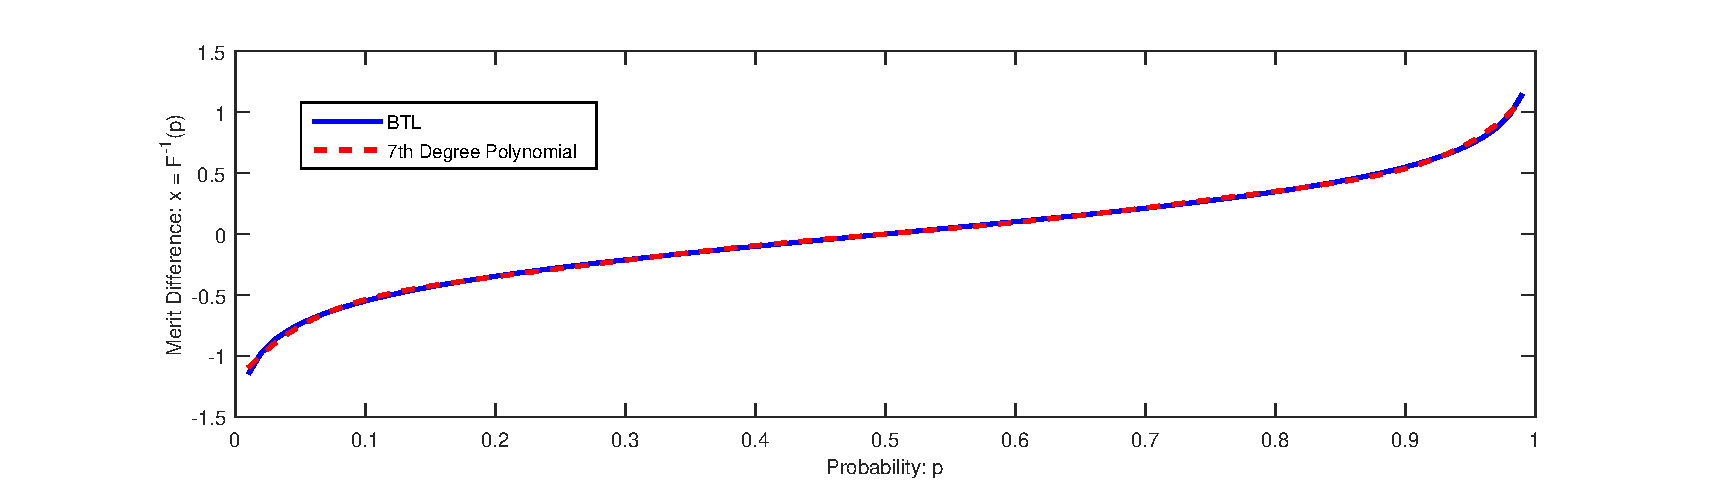
\includegraphics[width=1\textwidth]{BTL_polynomial_approx.eps}
    \caption{An  approximation of the Bradley-Terry-Luce quantile function over the interval $p\in[0.01, 0.99]$ by a function $F\in \mathcal{F}$ for $D = 7$. \label{fig:BTL_polyfit}}
\end{figure}

It is known that $F$ and $G$ are equivalent comparison functions iff $F(x) = G(\kappa x)$ for some positive $\kappa$, see \citet{yellott2}, and therefore $F^{-1}$ is equivalent to $G^{-1}$ iff  $\kappa F^{-1}(p) = G^{-1}(p)$.  A valid linear constraint on the coefficient vector $\boldsymbol{\beta}$ is thus imposed to ensure identifiability. For example, fixing the support of $F$, which amounts to fixing $\beta_0<0$, is sufficient. Another natural choice is to fix the derivative of $F$ at $0$, which amounts to fixing $\beta_1>0$. A rescaling argument shows that the resulting inferences do not depend on the chosen constraint. As noted earlier, identifiablity requires that the merits satisfy a constraint. Henceforth it will be assumed that: \\
\\
\textit{$\mathrm{A}_3$ (Scaling Assumption):} \textit{ The merits and the comparison function are scaled to satisfy}
\begin{equation}
\label{eq:additional_constraints}
\sum_i \mu_i = 0 \ \ \textit{ and } \ \ \beta_0 = -1.
\end{equation} 

Thus, if $F$ belongs to $\mathcal{F}$ we may estimate $(\boldsymbol{\mu},\boldsymbol{\beta} )$ by solving the following optimization problem:
\begin{equation}
\label{prob:semi_param_estimation}
(\boldsymbol{\hat  \mu}  ,  \boldsymbol{\hat \beta} ) \in \text{argmin}_{\boldsymbol{\mu} \in \mathbb{R}, F_{\boldsymbol{\beta}} \in \mathcal{F}}  ||F^{-1}_{\boldsymbol{\beta}} (\boldsymbol{\hat{P}}) - \Delta \boldsymbol{\mu} ||_{\Scale[.6]{\boldsymbol{W}}}.
\end{equation}
Although (\ref{prob:semi_param_estimation}) is a least squares problem it is non-standard as ``both sides", i.e., the ``predictor" and the ``response" in the regression equation, are associated with unknown parameters which are estimated simultaneously. In the following subsection we will study problem (\ref{prob:semi_param_estimation}) under assumptions $\mathrm{A}_1$ to $\mathrm{A}_3$.\\  
\\
\textit{Solution via Semidefinite Programming.} Our first concern is to characterize the set of feasible solutions for $(\boldsymbol{  \mu},\boldsymbol{\beta})$.  As noted earlier the quantile function (\ref{eq:F_inv}) satisfies $F^{-1}(p) = - F^{-1}(1-p)$ so we need only consider constraints generated by values $ p \in [0,1/2]$. In this interval $F^{-1}_{\boldsymbol{\beta}}(p)$ is increasing hence its derivative, which is a polynomial of degree $D-1$, is non-negative. Furthermore, the Lipschitz continuity constraint on $F$ implies that $F^{-1}$ is strictly monotone with derivative greater or equal to $1/L$. Thus,
\begin{equation}
\label{eq:constraints1}
    \beta_1 +...+ D \beta_D p^{(D-1)} - \frac{1}{L} \geq 0 \text{ for all } p \in [0,1/2] 
\end{equation}
 In addition $F(0) = 1/2$, so $F^{-1}_{\boldsymbol{\beta}}(1/2) = 0$ and  $||\boldsymbol{\beta}||_{\infty} \leq U$ therefore
\begin{equation}
\label{eq:constraints2}
     \sum_{i = 0}^D \left(\frac{1}{2}\right)^i \beta_i = 0
  \text{ and } -U \leq \beta_{i} \leq U \text{ for all } i. 
\end{equation}

Minimizing $||F^{-1}(\boldsymbol{\hat{P}}) - \Delta \boldsymbol{\mu}||_{\Scale[.6]{\boldsymbol{W}}}$ subject to (\ref{eq:constraints1}) and (\ref{eq:constraints2}) yields a  semi-infinite programming problem (SIP) \citep{mutapcic, stein}, i.e., an optimization problem with an infinite number of, in this case linear, constraints.  

There are a number of methods for solving SIPs. One natural approach is discretization, which in our case means replacing (\ref{eq:constraints1}) by $N$ constraints of the form $\beta_1 + \beta_2 p_j...+ D \beta_D p_j^{(D-1)} - 1/L \geq 0$ where $0<p_1 < p_2 <...< p_N< 1/2$ for some finite $N$. This yields a simple quadratic programming problem. From a practitioner's point of view, discretization may be a method of choice due to its simplicity.  This is specifically true when $||\cdot||_{\boldsymbol{W}}$ is either the weighted or unweighted $\mathcal{L}_1$ or $\mathcal{L}_{\infty}$ norms, since in these cases discretization results in a simple linear program. However, the resulting estimate of $F$ is not guaranteed to be strictly monotone (although this can be overcome, see section 3.2 of \citealt{mutapcic}) and more importantly in the worst case the solution may not be polynomially computable. 
These issues may be overcome by noting that the constraints in  (\ref{eq:constraints1})-(\ref{eq:constraints2}) are equivalent to a combination of linear constraints and positive semi-definite cone constraints, see  \citet{parrilo} for further details. Thus our optimization problem is (also) a semi-definite optimization problem (SDP). There is a large literature on SDPs \citep{nemirovski} and in particular it is known that SDPs can be solved by interior point methods \citep{vandenberghe} in polynomial time. Therefore we may formally rewrite (\ref{prob:semi_param_estimation}) as:

\begin{theorem}% [Problem Characterization]
\label{the:sdp_set}
Given $U,L\geq 0$, $D = 2d+1$ with $d\in \mathbb{N}$, a symmetric weight matrix $\boldsymbol{W}$ and an estimator $\boldsymbol{\hat P}$, then problem (\ref{prob:semi_param_estimation}) is equivalent to:
\begin{equation}
\label{SDP_characterization}
\begin{array}{lllllllll}
\text{minimize}  & \Scale[1]{\sum}_{(i,j)\in \mathcal{S}} \ w_{ij}(\beta_0 +  ... + \beta_D\hat{p}_{ij}^D +\mu_j- \mu_i )^2  \\
 %& \begin{array}{c} \Scale[0.3]{ i\neq j, \hat{p}_{ij} < \frac{1}{2}} \\  \Scale[0.3]{i<j, \hat{p}_{ij} = \frac{1}{2}}  \\ \end{array} \\
\text{subject to} \\
  &  \beta_{i} =  \frac{1}{i}(\frac{1}{2}t_{i-2} - t_{i-3} + s_{i-1})   \Scale[1]{\text{ for } i = 2,...,D},\\
  & \beta_{1}   = s_{0} +\frac{1}{L}, \ \ \ \ \sum_{k = 0}^D \left(\frac{1}{2}\right)^k \beta_k  = 0, \ \ \ \ \ \ ||\boldsymbol{\beta}||_{\infty} \leq U, \\

&   \\

& s_i =  \sum_{j+k = i}Q^0_{jk}   \Scale[1]{\text{ for } i = 0,...,D-1},  \ \ \ \  \boldsymbol{Q^0} \in \mathbb{S}_+^{d+1},\\
& t_i =  \sum_{j+k = i}Q^1_{jk}   \Scale[1]{\text{ for } i = 0,...,D-3},  \ \ \ \  \boldsymbol{Q^1} \in \mathbb{S}_+^{d}. \\
\end{array}
\end{equation}
where $\mathcal{S} = \{(i,j) \  | \ p_{ij} \leq .5 \text{ or } p_{ij} = .5 \text{ and } i<j\}$,  and  $t_{D-1}=t_{D-2}=t_{-1}=t_{-2}=0$, $\mathbb{S}_+^{k}$ is the set of $k\times k$ symmetric positive semi-definite matrices, and the rows and columns of $\boldsymbol{Q^0}$ and $\boldsymbol{Q^1}$ are indexed by $0$ to $d$ and $0$ to $d-1$ respectively. 
\end{theorem}

For brevity we present here only the case when $D$ is odd, a similar characterization holds for $D$ even. We note that analogues of Theorem \ref{the:sdp_set} could also be formulated for the  $\mathcal{L}_1$ and $\mathcal{L}_{\infty}$ norms and their weighted versions in which case the constraints in (\ref{SDP_characterization}) would remain unaltered whereas the objective function would be as defined by the corresponding norm.

Note that (\ref{SDP_characterization}) admits a unique solution when the objective function is positive definite. Lemma \ref{lem:weights_equal} below provides an example in a simple but important case. In large samples 
the solution to (\ref{SDP_characterization}) is uniquely determined when the system of equations $\beta_1 p_{ij}+...+\beta_D p_{ij}^D - (\mu_i -\mu_j)= -\beta_0$ for $(i,j)\in \mathcal{S}$ is of full rank. This condition is met when (i) there are at least $I+D-1$ connected pairs $(i,j)\in \mathcal{S}$; which (ii) the coefficients appearing in the linear equations, which are derived from the comparison probabilities $p_{ij}$, are sufficiently diverse, otherwise the resulting equations would not be linearly independent. Thus we assume that:\\
\\
\textit{$\mathrm{A}_4$ (Connectivity \& Diversity Assumption):} \textit{The comparison graph has at least $I+D-1$ edges. These edges correspond to a set of linearly independent equations of the form} $\beta_1 p_{ij}+...+\beta_D p_{ij}^D - (\mu_i -\mu_j)= -\beta_0$. \\

If we label these equations $(ij)_1,...,(ij)_{D+I-1}$ then together with the constraint $\sum \mu_i = 0$ we may write the resulting system of equations (with a slight abuse of notation) as:
\begin{equation}
\label{eq:linear_equation}
\boldsymbol{A} \left(\begin{array}{l}
     \boldsymbol{\beta}\\
     \boldsymbol{\mu} 
\end{array}\right) = \left(\begin{array}{c}
     -\boldsymbol{\beta_0} \\
     0
\end{array}\right)
\end{equation}
where the $k$'th row of $\boldsymbol{A}$ is $\boldsymbol{A}_k = (p_{(ij)_k} \ \ \Scale[.8]{...} \ \  p_{(ij)_k}^D\ \   -\boldsymbol{e}_{(ij)_k})$  for $k = 1,..., \Scale[.8]{I+D-1}$  and $\boldsymbol{A}_{I+D} = (\boldsymbol{0}^T \ \ \Scale[.8]{...} \ \  \boldsymbol{1}^T)$
where $\boldsymbol{e}_{ij}\in \mathbb{R}^{I}$ is defined by  $\boldsymbol{e}_{ij} \equiv \boldsymbol{e}_i - \boldsymbol{e}_j$, where $\boldsymbol{e}_i$ is the standard basis. The condition number of $\boldsymbol{A}$ plays a role in the quality of our estimators. 
 
Define $\boldsymbol{p} = (1,\  p, \ ...\ ,\  p^D)^T$ and note that if all the weights are equal then
\begin{equation}
\label{eq:closed_form_solution}
 \mu_i = \frac{1}{I}\sum_k F_{\boldsymbol{\beta}}^{-1}(p_{ik})  = \frac{1}{I}\sum_{(i,k)\in \mathcal{S}} F_{\boldsymbol{\beta}}^{-1}(p_{ik})-\frac{1}{I}\sum_{(i,k)\notin \mathcal{S}} F_{\boldsymbol{\beta}}^{-1}(p_{ki})
\end{equation}
 and thus we may eliminate $\boldsymbol{\mu}$ from (\ref{SDP_characterization})  by means of  equation (\ref{eq:closed_form_solution}). This considerably reduces the size of the SDP at hand when the number of items $I$ is larger than $D$. Algorithm \textsc{PolyRank} (displayed below) takes advantage of this. Furthermore:
\begin{lemma}
\label{lem:weights_equal}
When all weights $w_{ij}$ are equal, then, the objective function of problem (\ref{SDP_characterization}) is equivalent to minimizing $ \boldsymbol{\beta}^T \boldsymbol{M} \boldsymbol{\beta}$, where \begin{equation}
\label{eq:M}
\boldsymbol{M}  \equiv  \sum_{(ij)\in \mathcal{S}} \boldsymbol{v}_{(ij)}\boldsymbol{v}_{(ij)}^T\end{equation} and \ \ \ \ \ \ \ 
$\boldsymbol{v}_{(ij)} \equiv - I\boldsymbol{\hat p}_{ij} +\sum_{(ik)\in \mathcal{S}} \boldsymbol{\hat p}_{ik} - \sum_{(ik)\notin \mathcal{S}} \boldsymbol{\hat p}_{ki}  - \sum_{(jk)\in \mathcal{S}} \boldsymbol{\hat p}_{jk} + \sum_{(jk)\notin \mathcal{S}} \boldsymbol{\hat p}_{kj}. $
\end{lemma}
Hence the estimators can be efficiently calculated in three steps:

\newpage

\begin{framed}
 \textit{
\center \textbf{Algorithm: \textsc{PolyRank}} \\ 
\textbf{ \ } \\
Input:  $\boldsymbol{\boldsymbol{\hat P}} \in [0,1]^{I\times I}$  $D\in \mathbb{N}$ an odd number and $U,L \geq 0$.
\begin{enumerate}
	\item Preprocessing: $
    \text{Calculate }\boldsymbol{M} $ as in equation (\ref{eq:M});
	\item Functional Estimation: $
    \label{eq:functional_estimation}
    \boldsymbol{\hat{\beta}} \equiv \text{argmin }    \{ \boldsymbol{\beta}^T \boldsymbol{M} \boldsymbol{\beta} 
    \text{ subject to  }(\ref{SDP_characterization}) \text{ and } (\ref{eq:additional_constraints})\};
    $
	\item Merit Estimation: $
     \hat{\mu}_i   = \frac{1}{I}\sum_{(i,k)\in \mathcal{S}} F_{\boldsymbol{\hat \beta}}^{-1}(\hat{p}_{ik})-\frac{1}{I}\sum_{(i,k)\notin \mathcal{S}} F_{\boldsymbol{\hat\beta}}^{-1}(\hat{p}_{ki}); 
     $ 
     \end{enumerate}
\textbf{ \ }Output: $\boldsymbol{\hat \beta} \in \mathbb{R}^{D+1}$, $\boldsymbol{\hat \mu}\in \mathbb{R}^n$ and $\boldsymbol{P}^* \equiv F_{\boldsymbol{\hat \beta}}(\Delta \boldsymbol{\hat \mu})$
 }
\end{framed}

Step $1$ may be performed with no more than $O(I^3D+I^2D^2)$ operations, Step $2$ with no more than $O(D^2\sqrt{D})$ operations and Step $3$ with no more than $O(I^2D)$ operations. Thus, the overall computational complexity of solving problem (\ref{prob:semi_param_estimation}) is no more than $O(I^3D+I^2D^2+D^2\sqrt{D})$. Notice also that Steps 1 and 3 can be done in a distributed fashion. When the weights are not all equal the merits cannot be written as in (\ref{eq:closed_form_solution}) and therefore Algorithm \textsc{PolyRank} as stated above cannot be used, in that case we solve (\ref{SDP_characterization}) directly. Nevertheless we will refer to all versions of our estimation procedure as  \textsc{PolyRank}. In our experience, problem (\ref{prob:semi_param_estimation}) with any norm (weighted or unweighted) can be tackled successfully with a generic convex optimization solver on a desktop computer for problems of moderate size (e.g. with $D\leq 10$ and $I\leq 120$) in at most 2 or 3 seconds. Using the three step procedure (with the same generic solver) allows easy scaling up to problems where $D\leq 20$ and $I\leq 10000$. If  (\ref{prob:semi_param_estimation}) is treated as a SIP and solved via discretization, then significant reduction in computation time is observed at the cost of loosening the guarantee of optimality.

\paragraph{Remark 1} Notice that if the machine precision is $\epsilon$ and if $D$ is such that $\epsilon> (1/2)^D$ then the last terms of the polynomial $F^{-1}$ are rounded to zero. Therefore for standard 32 bit floating point arithmetic one should choose $D$ at most $22$, similarly for a 64 bit arithmetic $D$ should not surpass $44$. 
 $O(V^2\sqrt{V})$  
\paragraph{Remark 2} In theory $F$ can be recovered from  $F^{-1}$ exaclty via Lagrange Inversion Theorem. Numerically though, calculating $F_{\boldsymbol{\beta}}(\mu_i - \mu_j)$ reduces to a polynomial root-finding problem. Although root-finding is an ill-conditioned problem for general polynomials (Trefethen 2011), it may be solved via binary search  (with linear convergence in the worst case) or via Newton steps (with possible quadratic convergence).
\paragraph{Remark 3} When the weights $w_{ij}$ are not all equal, or $||\cdot||_{\boldsymbol{W}}$ represents the $\mathcal{L}_1$ or $\mathcal{L}_{\infty}$ norms, then a full SDP with $V = I+D$ variables must be solved. In these cases the simplifying row-sum structure is absent and the worst case bounds are well known, and of the order $O(V^2\sqrt{V})$, see the general SDP literature \citep{vandenberghe}. 

 
%{\color{red}\paragraph{Remark 3} Several applications may be interested solely on recovering the comparison function $F$. In such situations one need only perform steps 1 and 2 of \textsc{PolyRank}.}

\section{Sensitivity Analysis}
\label{sec:sensitivity_analysis}
%1. With known F;\\
%2. With unknown F:\\
%   a) Agnostic case;\\
%   b) Realizable case;\\ \\

The goal of this section is to  investigate the sensitivity of \textsc{PolyRank} with respect to the input matrix $\boldsymbol{\hat{P}}$. There are several reasons for developing thorough, non-stochastic, sensitivity bounds. Firstly, the analysis serves to clarify the mechanics of \textsc{PolyRank} providing bounds that apply to any choice of $\boldsymbol{\hat{P}}$. Secondly, using the sensitivity bounds statistical properties such as consistency of the refined estimator are easily derived. A third motivation is that different estimators $\boldsymbol{\hat P}$ have been investigated in the literature, e.g., \citet{rajkumar,chatterjee,shah}, and since \textsc{PolyRank} may be applied to any of them, the respective bounds on the refined estimator are universal and apply to any $\boldsymbol{\hat P}$. Sensitivity analysis is carried out under three increasingly general settings. First, we provide a benchmark by studying the LS method with known $F$. Then, we consider \textsc{PolyRank} in the case where the model is correctly specified, i.e., $F \in \mathcal{F}$. This is also called the realizable case. Finally, we consider agnostic cases, that is, situations where the model may be misspecified in some way. Three  examples of misspecifications are analyzed. 

For simplicity we first focus on the unweighted $\mathcal{L}_2$ norm, extensions to the respective weighted versions are similarly obtained.  

\subsection{Known Comparison Function}
%In this first scenario we consider is the case when function $F$ is  known. The purpose of this first analysis is to provide benchmarks for the more general and harder cases. 
Here the function $F$ is assumed to be a known $L$-Lipschitz continuous function with a $U$-Lipschitz inverse, i.e., it is bilipschitz. A common assumption in the literature, cf. \citet{shah2,shah}, is that the probabilities in  (\ref{eq:linear_model}) are bounded away from $0$ and $1$, i.e., $p_{ij} \in [\epsilon,  1-\epsilon]$, for some $\epsilon > 0$. Over this domain the Bradley-Terry-Luce, Thurstone, Threshold and Locally Linear models are all bilipschitz.
\begin{theorem}%[Sensitivity Analysis: Known $F$]
\label{the:sensitivity_LS}
Let $F$ be a known $L$-Lipschitz continuous function with a $4U$-Lipschitz continuous inverse (over their respective domains). Let $\boldsymbol{\hat \mu} $ be as in (\ref{prob:weighted_least_squares}) and $\boldsymbol{P^*} = F(\Delta \boldsymbol{\hat \mu})$. Then,  
\begin{equation}
\label{eq:prob_sens_known}||\boldsymbol{P^*} - \boldsymbol{P}||  \leq 4L U  ||\boldsymbol{\hat{P}} - \boldsymbol{P}||, \end{equation}
 and
 \begin{equation}
 \label{eq:merit_sens_known}|| \boldsymbol{\hat{\mu}} - \boldsymbol{\mu}||  \leq \frac{4U}{\sqrt{2I}}  || \boldsymbol{\hat{P}} - \boldsymbol{P}||.\end{equation}
If, additionally, it is assumed that $\boldsymbol{\hat P}$ obeys strong stochastic transitivity, then the estimators are order preserving, i.e.,
\begin{equation}\hat{\mu}_{i} < \hat{\mu}_{j} \iff \hat{p}_{ij} < \hat{p}_{ji}.\end{equation}
\end{theorem}

By construction the constant $4LU \geq 1$ and so (\ref{eq:prob_sens_known}) guarantees that $||\boldsymbol{P^*} - \boldsymbol{P}||$ will be at most a constant times $||\boldsymbol{\hat{P}} - \boldsymbol{P}||$. Although it may be possible to improve the constant in (\ref{eq:prob_sens_known}), its value can never be less than $1$, for if not, one could generate a converging sequence $\boldsymbol{P_{1}}^*$, $\boldsymbol{P_{2}}^*,...$ by recursively applying  the LS refinement to any initial (blind) guess of $\boldsymbol{\hat P}$. This argument holds for any refinement procedure,  including \textsc{PolyRank}. Also, by construction  the LS refinement defines $\boldsymbol{P}^*= F(\Delta \boldsymbol{\hat{\mu}})$ and thus $\min_{\boldsymbol{\mu}} ||F^{-1}(\boldsymbol{P}^*) - \Delta \boldsymbol{\mu}|| = 0$ for  $\boldsymbol{\mu}=\boldsymbol{\hat{\mu}}$ and so no improvement will be obtained via recursive LS type refinements. The bound in (\ref{eq:prob_sens_known}) is a ``worst case" bound and on average we often observe that $||\boldsymbol{P^*} - \boldsymbol{P}||$ is indeed smaller that $||\boldsymbol{\hat{P}} - \boldsymbol{P}||$. For  other norms refer to the appendix.

The benchmarks provided by Theorem \ref{the:sensitivity_LS} will be used for comparison with the more general cases tackled by \textsc{PolyRank}. As will be shown, inequality (\ref{eq:prob_sens_known}) also holds when $F$ is unknown (with different constant factors); similarly, the order preservation is maintained in all the settings considered.  

\subsection{Realizable Case} Under the hypothesis of  realizability, i.e., when the model is correctly specified, we have:

\begin{theorem}%[Sensitivity Analysis: Realizable Case]
\label{the:sensitivity_realizable}
Let $\boldsymbol{P^*} = F_{\boldsymbol{\hat{\beta}}}\left(\Delta \boldsymbol{\hat{\mu}}\right)$ where $\boldsymbol{\hat{\beta}}$ and $\boldsymbol{\hat{\mu}}$ are estimated using \textsc{PolyRank}. Then, 
  \begin{equation}
  \label{eq:sensitivity_realizable}||  \boldsymbol{P^*} - \boldsymbol{P}|| \leq (1+4LU)  ||\boldsymbol{\hat{P}} - \boldsymbol{P}||,\end{equation}
and 
\begin{equation}
\label{eq:parameter_sensitivity}\left|\left|\left(\begin{array}{c}
     \boldsymbol{\hat{\beta}} -\boldsymbol{\beta}\\
     \boldsymbol{\hat{\mu}} -\boldsymbol{\mu} 
\end{array}\right) \right|\right| \leq K_1 ||\boldsymbol{\hat{P}} - \boldsymbol{P}||,\end{equation}
as well as,
\begin{equation}
\label{eq:chebyshev_convergence}
\max_{x \in [-1,1] }|F_{\boldsymbol{\hat \beta}}(x) - F_{\boldsymbol{\beta}}(x)| \leq K_2 ||\boldsymbol{\hat{P}} - \boldsymbol{P}||_{\infty},
\end{equation}
where  $K_1 \leq U(1+4LU)\sqrt{D(I+D)} || \boldsymbol{A}^{-1}||$ and $K_2 \leq 16 LDU^2 \max_{i} \sum_j|A_{ij}^{-1}|$. If, additionally, it is assumed that $\boldsymbol{\hat P}$ obeys strong stochastic transitivity, then the estimators are order preserving.
\end{theorem}
Notice that the constants in (\ref{eq:prob_sens_known}) and (\ref{eq:sensitivity_realizable}) depend solely on the product of the Lipschitz constants of $F$ and $F^{-1}$. Moreover the constant in (\ref{eq:sensitivity_realizable}) does not depend on $D$ nor on the condition number of A . In contrast, the constants in inequalities (\ref{eq:merit_sens_known}) and (\ref{eq:parameter_sensitivity}) do depend on the dimensions of the problem. Equation (\ref{eq:chebyshev_convergence}) guarantees the convergence of $F_{\boldsymbol{\hat \beta}}$ to the true function $F$ with respect to the Chebyshev distance, thus, one can eventually recover $F$ with arbitrary precision. 

\subsection{Agnostic Cases}
We will now  investigate the properties of \textsc{PolyRank} under several types of misspecification. First, we investigate the effect of misspecifying the degree of the polynomial (\ref{eq:F_inv}). Then, we provide results analogous to those provided by Theorem \ref{the:sensitivity_realizable} by replacing the assumption that $F\in \mathcal{F}$ by the assumption that the true $F$ is an analytic function.  Finally, we drop the assumption that $\boldsymbol{P}$ satisfies the LST hypothesis all together and verify that we can still derive, albeit, weaker sensitivity bounds and rank consistency properties if strong stochastic transitivity is assumed.

\begin{theorem}% [Chebyshev Approximation Error]
\label{the:underfit}
Assume the true model satisfies (\ref{eq:F_inv}), however the fitted model was of degree $D' \leq D-1$. Then for any $\boldsymbol{\beta'}$ of dimension $D' \leq D-1$, a lower bound on the approximation error, in the Chebyshev norm, is:
%\begin{equation}
%\label{eq:underfit_1}
%    \max_{\alpha \in [0,1] }|F^{-1}_{\boldsymbol{\hat \beta}}(\alpha) - F^{-1}_{\boldsymbol{\beta}}(\alpha)| \geq 2 \frac{|\beta_{D}|}{8^D}
%\end{equation}
\begin{equation}
\label{eq:chebyshev_bad}
    \frac{1}{2 U} \frac{|\beta_{D}|}{8^D} \leq \max_{\alpha }|F_{\boldsymbol{\beta'}}(\alpha) - F_{\boldsymbol{\beta}}(\alpha)|  
\end{equation}
\end{theorem}

The lower bound (\ref{eq:chebyshev_bad}) shows that the Chebyshev distance between the true function and the estimated function cannot be arbitrarily minimized when the degree of the fitted polynomial is under-specified. The lower-bound, though, decreases with the value of $D$ at an exponential rate.

\begin{theorem}%[Sensitivity Analysis - Analytic Case]
\label{the:analytic_sensitivity_LS}
Let $\boldsymbol{P^*} = F_{\boldsymbol{\hat{\beta}}}\left(\Delta \boldsymbol{\hat{\mu}}\right)$ where $\boldsymbol{\hat{\beta}}$ and $\boldsymbol{\hat{\mu}}$ are estimated with \textsc{PolyRank}. Assume that the true probability matrix $\boldsymbol{P} = F(\Delta \boldsymbol{\mu})$ for some $\boldsymbol{\mu}$ and some unknown $L$-Lipschitz continuous function $F$ with an analytic inverse function $F^{-1}$ whose coefficients are upper-bounded by $U$. Then for the estimated probability matrix we have:
\begin{equation}
\label{eq:analytic_sensitivity}
||\boldsymbol{P^*} - \boldsymbol{P}||\leq (1+4LU)||\boldsymbol{\hat{P}} - \boldsymbol{P}||  + \frac{1}{2^D}LUI 
\end{equation}
If additionally it is assumed that $\boldsymbol{\hat P}$ obeys strong stochastic transitivity, then the estimators are order preserving.
\end{theorem}

Equation (\ref{eq:analytic_sensitivity}) shows that the error of $\boldsymbol{P}^*$ can be controlled under a broad class of analytic functions. The first term is controlled by increasing the precision of $\boldsymbol{\hat P}$ and the second term is controlled by choosing larger values for $D$. 


In the following Theorem we will assume no particular structure on $\boldsymbol{P}$, i.e. the probability matrix $\boldsymbol{P}$ need not be consistent with any stochastic transitivity model. %This is our final and harshest condition under which we investigate the sensitivity of \textsc{PolyRank}.

\begin{theorem}%[Sensitivity Analysis - Full Agnostic Case]
\label{the:agnostic_sensitivity}
Let $\boldsymbol{P^*} = F_{\boldsymbol{\hat{\beta}}}\left(\Delta \boldsymbol{\hat{\mu}}\right)$ where $\boldsymbol{\hat{\beta}}$ and $\boldsymbol{\hat{\mu}}$ are  estimated with \textsc{PolyRank}. Then for the estimated probability matrix we have:
%, then the difference between the true loss and the empirical loss is no more than a constant times $||\boldsymbol{\hat{P}} - \boldsymbol{P}||$; that is: %\begin{equation}\left| \ \  \left|\left|F^{-1}_{\boldsymbol{\hat \beta}}(\boldsymbol{\hat{P}}) - \Delta \boldsymbol{\hat\mu}\right| \right|  - \left|\left|F^{-1}_{\boldsymbol{\hat \beta}}(\boldsymbol{P}) - \Delta \boldsymbol{\hat\mu}\right| \right| \ \ \right| \leq K||\boldsymbol{\hat{P}} - \boldsymbol{P}||\end{equation}
%where $K  \leq 4  ||\boldsymbol{\hat \beta}||_{\infty}\leq 4  U$.
\begin{equation}
\label{eq:agnostic_sensitivity}
||\boldsymbol{P}^* - \boldsymbol{P}|| \leq ||\boldsymbol{\hat P} -\boldsymbol{P}|| + L ||F^{-1}_{\boldsymbol{\hat \beta}}(\boldsymbol{\hat{P}}) - \Delta\boldsymbol{\hat \mu}||,
\end{equation}
If additionally it is assumed that $\boldsymbol{\hat P}$ obeys strong stochastic transitivity, then the estimators are order preserving.
\end{theorem}
%\sketchproof
%$\left| \ \ \left|\left|\left(F^{-1}_{\boldsymbol{\hat \beta}}(\boldsymbol{P}) - \Delta \boldsymbol{\hat\mu}\right)\right| \right|_{2} - \left|\left|\left(F^{-1}_{\boldsymbol{\hat \beta}}(\boldsymbol{\hat{P}}) - \Delta \boldsymbol{\hat\mu}\right)\right| \right|_{2} \ \ \right|   $
%$$\leq_{[1]} || F^{-1}_{\boldsymbol{\hat \beta}}(\boldsymbol{P}) - F^{-1}_{\boldsymbol{\hat \beta}}(\boldsymbol{\hat{P}}) ||_2 \leq_{[2]} \sqrt{\sum_{ij} \mathcal{L}_{\boldsymbol{\hat \beta}}^2 \left( P_{ij}-\hat{P}_{ij} \right)^2}$$ 
%[1] Every norm is $1-$Lipschitz continuous with respect to itself.
%[2] $F^{-1}_{\boldsymbol{\hat \beta}}(p)$ is $\mathcal{L}_{\boldsymbol{\hat \beta}}-$Lipschitz continuous (to see this use the mean value theorem).
%\qed
An immediate consequence of order preservation is that if  $\boldsymbol{P}$ is in the interior of the strong stochastic transitivity set then \textsc{PolyRank} is order-consistent for any consistent estimator $\boldsymbol{\hat P}$, i.e., when $\boldsymbol{\hat P}\to \boldsymbol{P}$ then the vector  $\boldsymbol{\hat{\mu}}$ will correctly recover the underlying order among the items. The error bound in equation (\ref{eq:agnostic_sensitivity}), though, cannot be controlled as in equation (\ref{eq:analytic_sensitivity}), this is so because the second term can be as big as $\kappa I^2$ for some positive $\kappa$ even when $\boldsymbol{\hat P}$  satisfies  strong stochastic transitivity  \citep{shah}.

\section{Convergence and Concentration}
\label{sec:statistical_properties}
%1. Consistency with polynomial $F^{-1}$;\\
%2. Case studies:   Round-Robin Case \& Blind Case;\\ \\
%3. Variance of least squares\\ \\

In this subsection we assume that the model is correctly specified and investigate some properties of the estimators obtained by \textsc{PolyRank}. We start with the case where the comparisons graph is fixed and the number of comparisons per pair, i.e., the $m_{ij}$'s is allowed to increase. Similar conditions have been considered in literature \citep{rajkumar,shah2}. 

%Under this setting we investigate the quality of our estimator with respect to the number of paired comparisons and the topology.

It is well known that the topology of the comparison graph plays an important role in the quality of the estimators \citep{shah2, massey, colley}. In particular \citet{shah2} show that, the mean squared errors of the estimated merits from a standard Bradley-Terry-Luce model are proportional to the second eigenvalue of the graph Laplacian. This eigenvalue, referred to as the algebraic connectivity of the graph, measures how ``well" the graph is connected \citep{chung2}. In our concentration bounds the number of edges in the comparison graph and the condition number associated with (\ref{eq:linear_equation}) will play a similar role. Let  $n = \sum_{i,j} m_{ij} $ be the number of paired comparisons.

\begin{theorem}%[Hoeffding: Realizable Case]
\label{the:hoeffding_realizable}
Let $\boldsymbol{\hat{\beta}}_n$ and $\boldsymbol{\hat{\mu}}_n$ be estimated using \textsc{PolyRank} with $m_{ij} \equiv w_{ij} n$. Let $\hat{p}_{ij}$ be the usual MLEs. Then for large enough $n$ there are constants $K_1$ and $K_2$ such that, 
\begin{equation}
\label{eq:hoeffding_realizable}
\mathbb{P}\left(\Scale[.9]{\left|\left|\left(\begin{array}{c}
     \boldsymbol{\hat{\beta}}_n -\boldsymbol{\beta}\\
     \boldsymbol{\hat{\mu}}_n -\boldsymbol{\mu} 
\end{array}\right) \right|\right|}\geq \epsilon \right) \leq K_1\exp\left(-n K_2   \epsilon^2 \right),\end{equation}
where $K_1$ and $K_2 $ are discussed bellow. 
\end{theorem}

Theorem \ref{the:hoeffding_realizable} shows that the estimators $\boldsymbol{\hat{\beta}}_n$ and $\boldsymbol{\hat{\mu}}_n$ converge at an exponential rate and are therefore strongly consistent. Theorem \ref{the:hoeffding_realizable} also implies an exponential convergence of $\boldsymbol{P}^*$ to $\boldsymbol{P}$ as well as of $F_{\boldsymbol{\hat \beta}}(x)$ to $ F_{\boldsymbol{ \beta}}(x)$ in the Chebyschev distance. Theorem \ref{the:hoeffding_realizable} is proved by first establishing sensitivity bounds for the weighted norm. These are analogues of Theorem \ref{the:sensitivity_realizable} and are of the form
\begin{equation}
\label{eq:weighted_parameter_sensitivity}\left|\left|\left(\begin{array}{c}
     \boldsymbol{\hat{\beta}} -\boldsymbol{\beta}\\
     \boldsymbol{\hat{\mu}} -\boldsymbol{\mu} 
\end{array}\right) \right|\right| \leq K ||\boldsymbol{\hat P} - \boldsymbol{P}||_{\Scale[.6]{\boldsymbol{W}}}.\end{equation}

The constants in (\ref{eq:hoeffding_realizable}) are $K_1 = 2|E|$ where $|E|$ is the number of edges in the comparison graph, and 
$K_2 = 2/(|E|(1+4LU)^2U^2D(I+D)||\boldsymbol{A}^{-1}_{\Scale[.6]{\boldsymbol{W}}}||^2)$, where $\boldsymbol{A}^{-1}_{\Scale[.6]{\boldsymbol{W}}}$ is defined as in equation (\ref{eq:linear_equation}) with the appropriate modifications for weights. Clearly, $I+D-1 \leq |E| \leq (I^2-I)/2$. Of course, smaller values of $|E|$ will provide tighter bounds in equation (\ref{eq:hoeffding_realizable}). The value of $|| \boldsymbol{A}_{\Scale[.6]{\boldsymbol{W}}}^{-1}||$ is a function of, among other things, the topology of the comparison graph. Unfortunately, the condition number of $A_{\Scale[.6]{\boldsymbol{W}}}$ is difficult to analyze as it contains a $(I+D-1) \times D$ Vandermonde submatrix which can range from $1$ (the best possible condition number) to exponential on the dimensions of the matrix \citep{pan}. As a rule of thumb Vandermonde matrices are well conditioned when the points $p_{(ij)_1},...,p_{(ij)_{D+I-1}}$ are (approximately) spaced over Chebyshev points. Matrix  $\boldsymbol{A}_{\Scale[.6]{\boldsymbol{W}}}$ also contains a standard $(I+D-1)\times I$ submatrix of pairings and thus we conjecture that smaller values of the second eigenvalue of the graph Laplacian matrix should also provide tighter estimation bounds.



%When the topology is pre-determined the pairs with $w_{ij}>0$ are fixed. This leads us to our next result with a setting analogous to that studied in \citep{shah2}. Here a weighted graph of paired comparisons is chosen arbitrarily and the number of matches per pair $m_{ij}$ increase proportionally  to the square of the weights $w_{ij}$ associated to its corresponding edge.

\subsection{Round robin} We now turn our attention to round robin tournaments \citep{chatterjee,shah,simons}, in which each pair of items is compared $m$ times. If the number of items $I$ is fixed and if $m \to \infty$ then we can use the results described above. A more interesting situations arises when $m=1$ but the number of items $I \to \infty$. As pointed out earlier, in this setting if  $\hat{p}_{ij} \propto Y_{ij}$ then the LS estimator $\hat{\mu}_i$ will be proportional to its Copeland Score (the number of times an item was preferred). Recent papers addressing this setting are by \citet{chatterjee} and \citet{shah}. In particular  they  assume strong stochastic transitivity and construct an estimator $\boldsymbol{\hat P}_{\text{ISO}}$ which is shown to satisfy: 
\begin{equation}
\label{eq:chatterjee}
	\sup \frac{1}{I^2} \mathbb{E} ||\boldsymbol{\hat P}_{\text{ISO}} - \boldsymbol{P} ||_2^2 \leq C    \sqrt{\frac{\log I}{I}},
\end{equation}
where the supremum is taken over all matrices that satisfy strong stochastic transitivity. They also show that if the true model was LST then, under some regularity conditions, the upper bound in (\ref{eq:chatterjee}) can be tightened to $O(1/I)$ up to log factors \citep{shah}. Their estimator is calculated in  two steps: (\textit{i}) first, they sort the items according to their Copeland Score; (\textit{ii}) then, they perform a two dimensional isotonic regression on the matrix $\boldsymbol{Y}$ assuming the order obtained in (\textit{i}). 

The resulting estimator has two drawbacks when the true model is LST. First, the estimator may be infeasible, i.e., $\boldsymbol{\hat P}_{\text{ISO}}$ may not be LST. Our experience indicates that this is frequently the case. In addition the resulting estimator does not fully exploit the benefits of an LST model since the estimated probability matrix is not a Functional of a merit vector and the comparison function. These deficiencies, however, can be addressed by applying \textsc{PolyRank} to their estimator. A trivial consequence of equation (\ref{eq:sensitivity_realizable}) is that the refined estimator $\boldsymbol{P}^*$ retains the optimal risk bounds of $\boldsymbol{\hat{P}}_{\text{ISO}}$ and by construction is feasible. We state the full result for completeness:

\begin{theorem} 
\label{the:RSS_ISO_SP}
Let $\boldsymbol{P}^*$  be the refinement of  $\boldsymbol{\hat{P}}_{\text{ISO}}$ using \textsc{PolyRank}, where $\boldsymbol{\hat{P}}_{\text{ISO}}$ is the estimator of \citet{chatterjee}, then:
\begin{equation}
	\sup \frac{1}{I^2} \mathbb{E} ||\boldsymbol{P}^* - \boldsymbol{P} ||_2^2 \leq K  \frac{\log^2 I}{I},
\end{equation}
for some constant $K $ that does not depend on neither $I$ nor $D$ (nor the condition number of $A$) and the supremum is taken over the set of probability matrices consistent with functions $F \in \mathcal{F}$. This is optimal up to log factors. 
\end{theorem}


\section{Numerical Experiments and An Illustrative Example}
\label{sec:numerical_experiments}


%\subsection{Simulations}
In the following we describe four experiments performed to further test and  investigate \textsc{PolyRank}. Each simulation is performed 1000 times and we report  and discuss  the average performance under the specified conditions.

\paragraph{Experiment 1:}  In this experiment we compare  the empirical performance of the estimator of $\boldsymbol{P}$ when using \textsc{PolyRank} with a low degree polynomial with its performance given the correct comparison function. Specifically, this is done by generating $I = 20$ items with merits $\mu_i$ sampled uniformly from $ [0, 10]$. A total of $50$ pairs, selected randomly, were compared assuming a Bradley-Terry-Luce (BTL) model. We refine the estimator $\hat{p}_{ij} = (Y_{ij}+1)/(m_{ij}+2)$ with \textsc{PolyRank} using $D=5$. We also compute the LS estimated with the known $F$.  Figure \ref{fig_refinement_comparisons} shows the  average distance $||\boldsymbol{P}^* - \boldsymbol{P}||_2$. As expected, the LS method with the correct comparison function performs best, \textsc{PolyRank} performs almost as well and both substantially outperform the initial estimates.  This is consistent with our expectations because the BTL model, despite not belonging to the class of functions $\mathcal{F}$, can be well approximated by this class within the range of choice probabilities generated.  
\begin{figure}
  \centering
    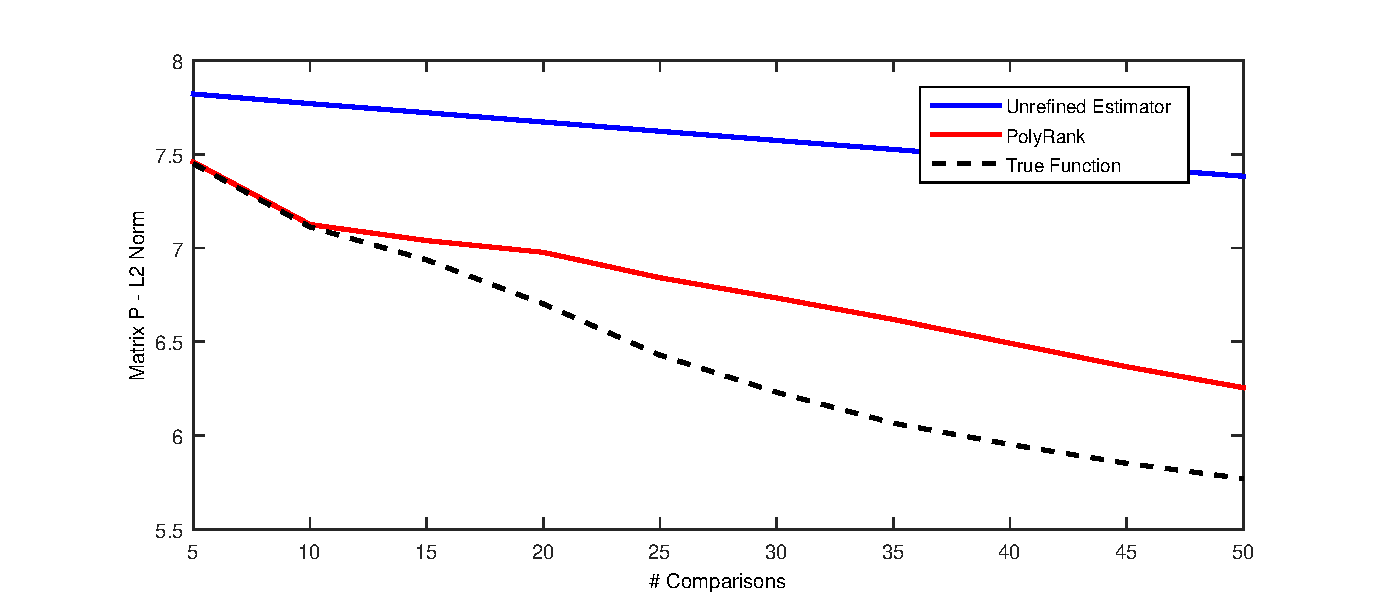
\includegraphics[width=1\textwidth]{refinement_comparisons.eps}
    \caption{Comparison of refined estimators with low sampling. \label{fig_refinement_comparisons}}
\end{figure}

%The maximum number of paired comparisons in this experiment was  less than $\lceil 20\log_2 20 \rceil = 87$, and the pairs were not chosen adaptively. Under these  harsh conditions, the weighted refinement procedures (with or without knowing $F$), perform better than the unrefined estimator. Notice that the  LS method with full knowledge of $F$ has only a slight increase in precision when compared to  \textsc{PolyRank}. 

\paragraph{Experiment 2}  In this experiment we investigate the empirical performance of \textsc{PolyRank} in the round-robin setting when the number of items is increasing. Specifically, we generate a sequence of round-robin tournaments with an increasing number of items. The data is generated assuming model (\ref{eq:F_inv}) with $D=5$. The matrix $\boldsymbol{P}$ is estimated using the isotonic regression estimator of \citet{chatterjee} and refined using  \textsc{PolyRank} with $D \in \{3,5,7\}$.  Figures \ref{fig:round_robin} and \ref{fig:round_robin_parameters} display, respectively, the average of $||\boldsymbol{P}^* - \boldsymbol{P}||^2/I^2$ and the average of $||(
     \boldsymbol{\hat{\beta}} -\boldsymbol{\beta},
     \boldsymbol{\hat{\mu}} -\boldsymbol{\mu}) ||^2/(I+D)$ for $I = 10, 20, 30, 40$ and $50$.

\begin{figure}
  \centering
    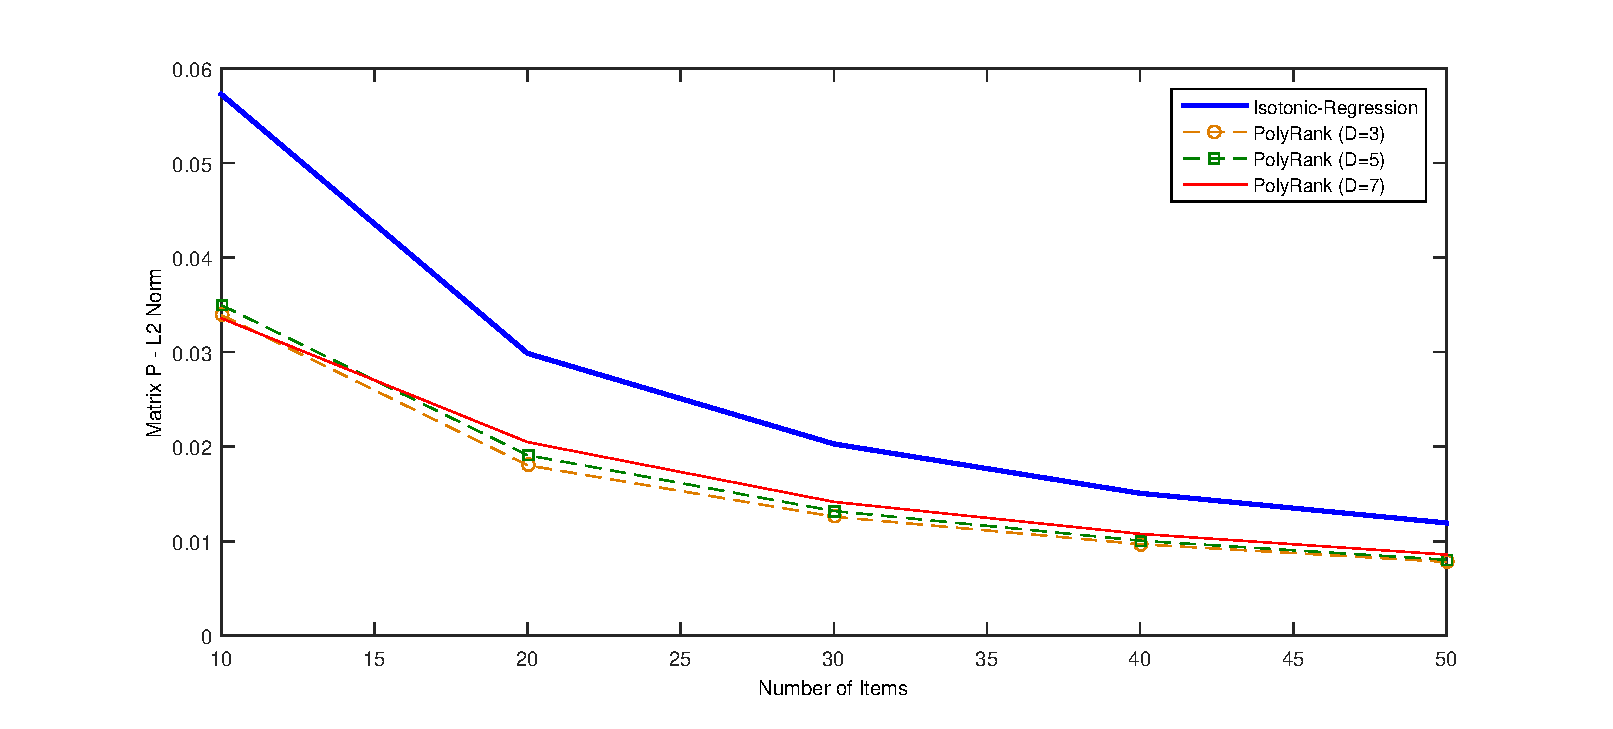
\includegraphics[width=1\textwidth]{round_robin_realizable}
    \caption{Refined estimators for round-robin tournaments. \label{fig:round_robin}}
\end{figure}


\begin{figure}
  \centering
    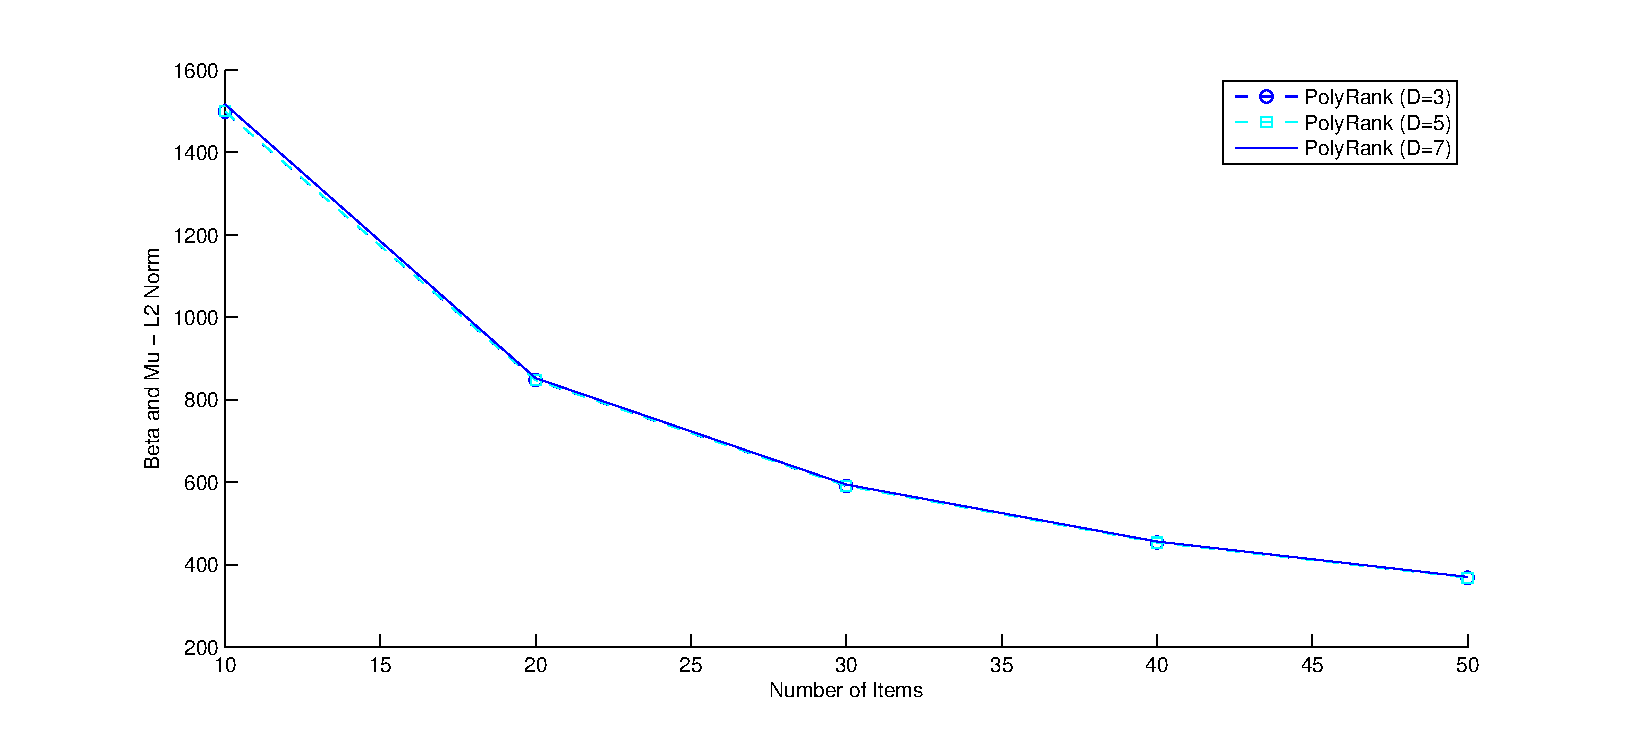
\includegraphics[width=1\textwidth]{round_robin_parameters}
    \caption{Estimated parameters for round-robin tournaments. \label{fig:round_robin_parameters}}
\end{figure}

Figure \ref{fig:round_robin} shows four curves, all of which decrease with $I$. The top curve is the risk for the unrefined isotonic-regression based estimator. The estimators refined by \textsc{PolyRank}, which correspond to the lower 4 curves always do better. Notice that over-fitting, i.e., $D=7$, which corresponds to the second curve from the top, usually results in higher estimation error with no change in the approximation error when compared to $D=3,5$. The second curve from the bottom corresponds to the true model. The bottom curve is obtained when $D=3$, i.e., under under-fitting, and results in the lowest risk. Although this result is somewhat surprising it has been documented also in the context of other models \citep[Chapter 5]{claeskens}. This indicates that lower degree polynomial often perform well in practice. In Figure \ref{fig:round_robin_parameters} we see that the average error of the estimated parameters decreases as a function of $I$.


\paragraph{Experiment 3:} In this experiment we investigate the performance of  \textsc{PolyRank} in the round-robin setting with a fixed number of items and a increasing number of comparisons. we generated a sequence of round-robin tournaments with $I=10$ and an increasing number of matches. The data is generated assuming model (\ref{eq:F_inv}) with $D=3$. The matrix $\boldsymbol{P}$ is estimated using the standard frequency estimator for $\hat{p}_{ij} $   and is refined using  \textsc{PolyRank} (with $D=3$). Figure \ref{fig:var_round_robin} displays the average of $||\boldsymbol{P}^* - \boldsymbol{P}||^2/I^2$, of $||\boldsymbol{\hat \mu} - \boldsymbol{\mu}||^2/I$ and of $||\boldsymbol{\hat \beta} - \boldsymbol{\beta}||^2$ for $m_{ij}  = 1$ to $5$ for all pairs $(i,j)$ and Figure \ref{fig:round_robin_function} shows the sequence of estimated functions.

The three decreasing curves of Figure \ref{fig:var_round_robin} show that the variance of the estimators decreases with the amount of paired comparisons. Figure \ref{fig:round_robin_function} shows that the estimated comparison function converges to its true value. These results and those of Experiment 2 are consistent with Theorems \ref{the:hoeffding_realizable} and \ref{the:RSS_ISO_SP}.

\begin{figure}
  \centering
    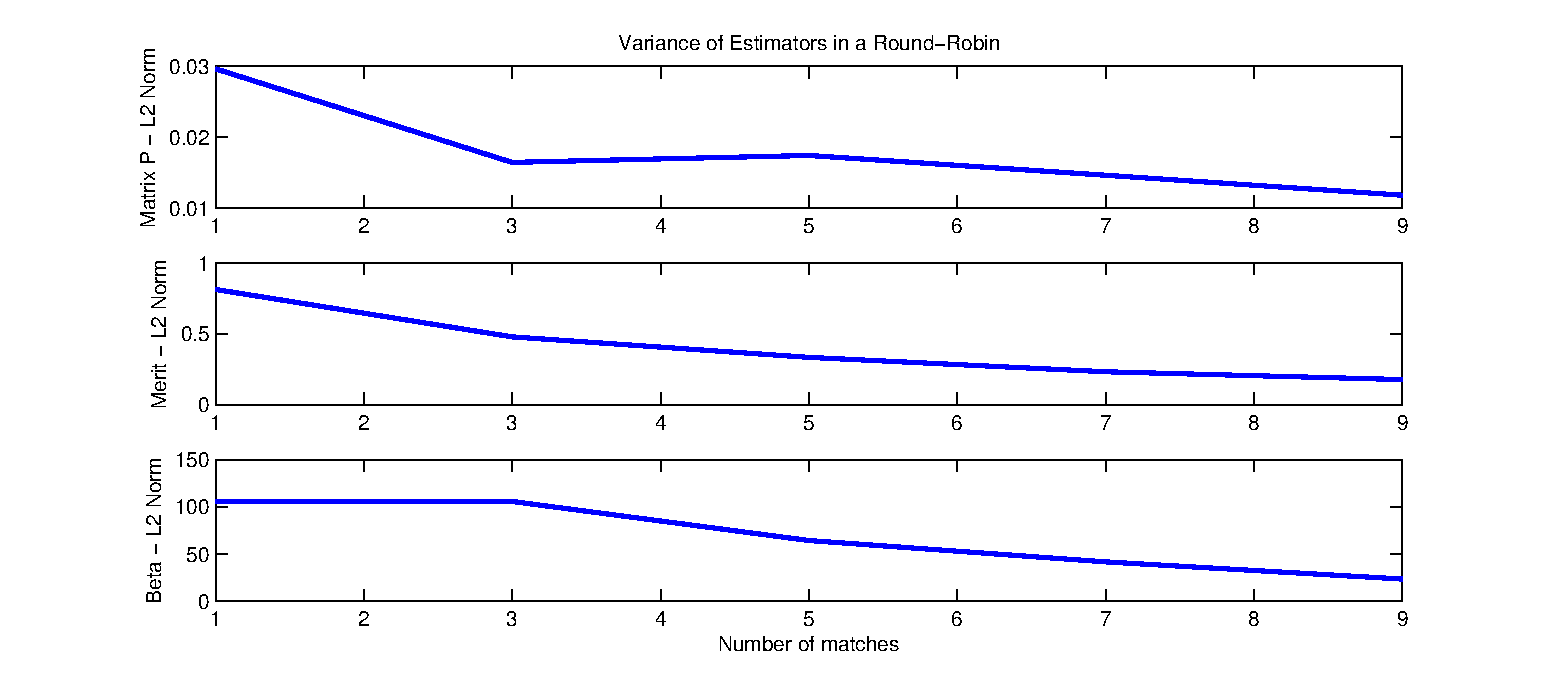
\includegraphics[width=1\textwidth]{variance_estimators_round_robin}
    \caption{Variance of estimators in a round-robin with increasing number of matches between each pair. \label{fig:var_round_robin}}
\end{figure}

\begin{figure}
  \centering
    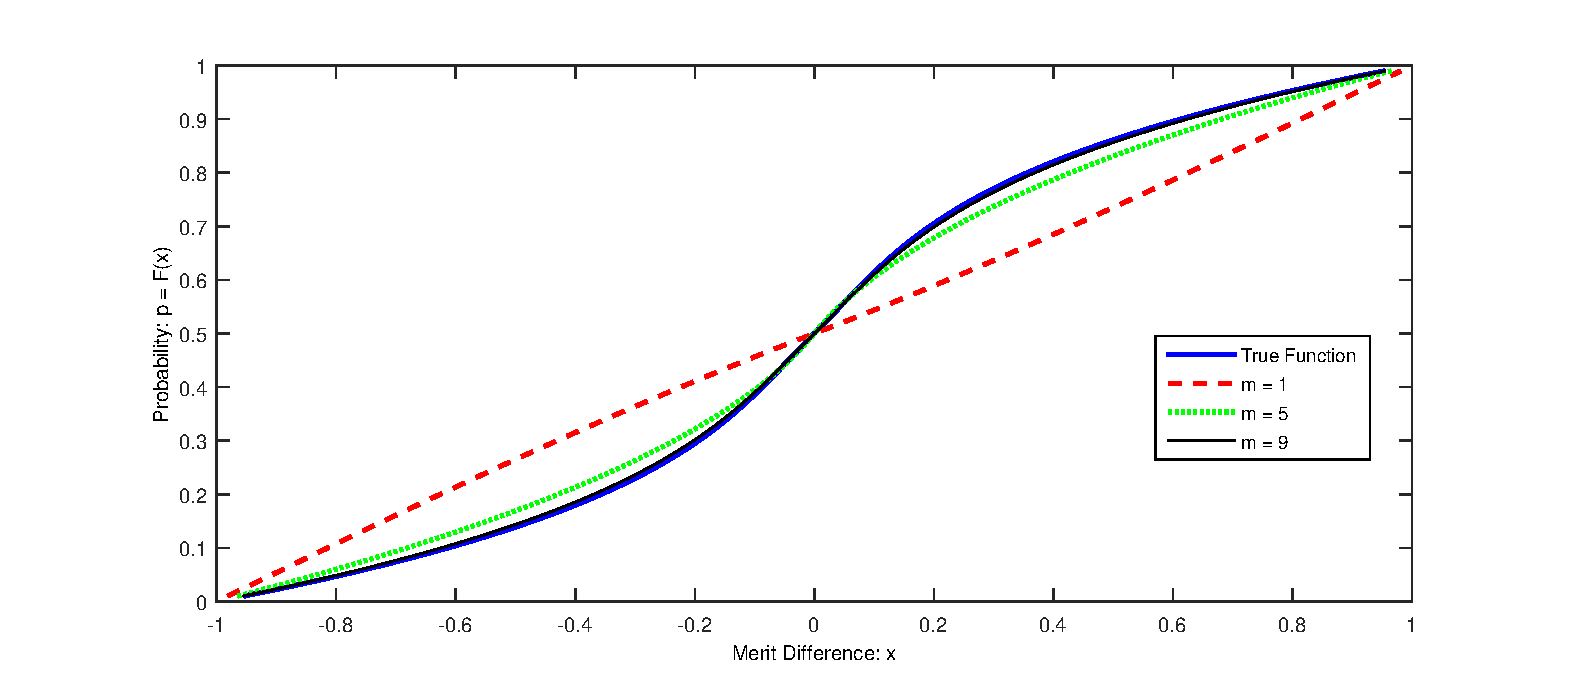
\includegraphics[width=1\textwidth]{round_robin_function_graph}
    \caption{Recovered function graph. \label{fig:round_robin_function}}
\end{figure}

\paragraph{Experiment 4:}
%\label{sec:model_selection}

In practice the degree $D$ of the polynomial (\ref{eq:F_inv}) may not be known in advance. If we choose $D$ to be too small then we may not fully capture the geometry of $F$, while if $D$ is too large there is a danger of over-fitting and possible numerical problems. In this  experiment we investigate the use of some well known model selection criteria \citep{claeskens} for choosing $D$. In particular, we test the empirical performance of the Bayesian Information Criterion (BIC) and two variants of the Akaike Information Criterion (AIC)  and contrast these with the performance of (leave-one-out) cross-validation. The classical AIC criteria is 

\begin{equation}
\label{eq:AIC}
\mathcal{AIC}(D) \equiv 2(I+D)+n\log(l(D))
\end{equation}
where $l(D)$ is the least-squares loss function, given in   (\ref{prob:semi_param_estimation}) and evaluated at  the estimated parameters, $I+D$ is the number of parameters in the model and $n$ is the sample-size. The corrected AIC (AICc) is 

\begin{equation}
\label{eq:AICc}
\mathcal{AIC}_c(D) \equiv \mathcal{AIC}(D) + \frac{2(I+D+1)(I+D+2)}{n-I-D-2}
\end{equation}
and is designed to correct for small sample-sizes. The BIC method penalizes more the number of parameters and is defined by
\begin{equation}
\label{eq:BIC}
\mathcal{BIC}(D) \equiv (I+D)\log(n)+n\log(l(D)).
\end{equation}

Tables \ref{tab:model_selection} and \ref{tab:model_selection2} compares the AIC, the AICc and the BIC methods in a round-robin data generated with $I=6$ and $I = 12$ objects and with $m_{ij} = 1$ for all $ij$, as well as $m_{ij} = 3$.  The data was generated  monotone polynomials of degree $5$ randomly selected with uniform coefficients and projected to the monotone cone. We display the frequency in which the methods correctly identify the degree of the polynomial as opposed to overfit/underfit.

\begin{table}[]
\centering
\begin{tabular}{ccccccccccccc}
        & CV & AICc    & AIC     & BIC   & & CV & AICc     & AIC       & BIC \\
$D = 1$ &       $100\%$    & $100\%$ & $100\%$ & $100\%$& &     $22\%$      & $30.3\%$ & $24.4\%$  & $37.4\%$\\
$D = 3$ &       $0\%$      & $0\%$   & $0\%$   & $0\%$  & &     $63.7\%$    & $67.3\%$  & $69.8\%$ &$61.6\%$\\
$D = 5$ &       $0\%$      & $0\%$   & $0\%$   & $0\%$  & &     $11.8\%$    & $1.5\%$    & $4.9\%$ & $0.1\%$\\
$D = 7$ &       $0\%$      & $0\%$   & $0\%$   & $0\%$  & &     $2.4\%$      & $0.8\%$  & $0.8\%$ & $0.8\%$ \\
$D = 9$ &       $0\%$      & $0\%$   & $0\%$   & $0\%$  & &     $0.1\%$      & $0.1\%$ & $0.1\%$  & $0.1\%$     \\  \cmidrule{2-5}  \cmidrule{7-10} \\ & \multicolumn{4}{c}{$m_{ij}= 1$}  & & \multicolumn{4}{c}{$m_{ij}= 3$}
\end{tabular} 
\caption{Model Selection ($I = 6$, $D = 5$)}
\label{tab:model_selection}
\end{table}

\begin{table}[]
\centering
\begin{tabular}{ccccccccccccc}
        & CV & AICc    & AIC   & BIC      & &CV & AICc   & AIC      & BIC   \\
$D = 1$ &       $100\%$    & $100\%$ & $100\%$ & $100\%$& &     $7.1\%$      & $2.8\%$  & $2.6\%$&$6.8\%$ \\
$D = 3$ &       $0\%$      & $0\%$   & $0\%$  & $0\%$   & &     $87.4\%$     & $89\%$ & $85.2\%$ &$92.5\%$\\
$D = 5$ &       $0\%$      & $0\%$   & $0\%$   & $0\%$  & &     $5.3\%$      & $8.2\%$ & $12.2\%$& $0.7\%$ \\
$D = 7$ &       $0\%$      & $0\%$   & $0\%$   & $0\%$  & &     $.2\%$       & $0\%$ & $0\%$ & $0\%$ \\
$D = 9$ &       $0\%$      & $0\%$   & $0\%$  & $0\%$   & &     $0\%$        & $0\%$ & $0\%$  & $0\%$ \\  \cmidrule{2-5}  \cmidrule{7-10}\\
& \multicolumn{4}{c}{$m_{ij}= 1$}  & & \multicolumn{4}{c}{$m_{ij}= 3$}
\end{tabular}
\caption{Model Selection ($I = 12$, $D=5$)}
\label{tab:model_selection2}
\end{table}
Tables \ref{tab:model_selection} and \ref{tab:model_selection2}  show the empirical performance of the model selection criteria as a function of number of items $I$ and the number of paired comparisons $m_{ij}$. For low values of $m_{ij}$ all criteria select the lowest degree polynomial, i.e., $D=1$. When the number of comparisons increases the procedures tend to select larger values of $D$. In general the performance of the procedures are comparable. However, AIC and Cross validation do seem to (slightly) outperform the other methods. Cross validation is significantly more demanding computationally than AIC and thus as a rule of thumb we recommend the use of the AIC method when no further information is available.

\subsection{Illustrative Example}

In this subsection we illustrate the use of \textsc{PolyRank} on a computer-chess data set\footnote{Publicly available at \url{http://kirill-kryukov.com/chess/kcec/games.html}.}. The data set comprises of matches between $186$ free single-CPU chess-engines. Each chess-engine played (roughly) $32$ matches against $40$  opponents. We use \textsc{PolyRank} to estimate model parameters from observed matches that resulted in a victory or defeat; ties are ignored. Figure \ref{fig:chess_more_dimensions} shows the estimated comparison function for various values of $D$ when  for the first 100 chess-engines. As is observed the estimated function $F_{\boldsymbol{\hat \beta}}$ seems to stabilize for  $D$ greater than or equal to $7$. Figure \ref{fig:chess_more_data} shows the estimated function when the dimension $D = 7$ is fixed and the number of chess-engines $I$ is gradually increased. For $I$ greater than or equal to $60$ our estimated function seems to stabilize. Finally, Figure \ref{fig:polyrank_vs_BTL} compares the best fit function recovered by \textsc{PolyRank} to the family of BTL models described by $F_{\text{BTL}}(x) = 1/(1+\exp(-\kappa x))$ for various values of $\kappa >0$. Somewhat surprisingly, it seems that the family of BTL functions  does not provide a good fit.

\begin{figure}
  \centering
    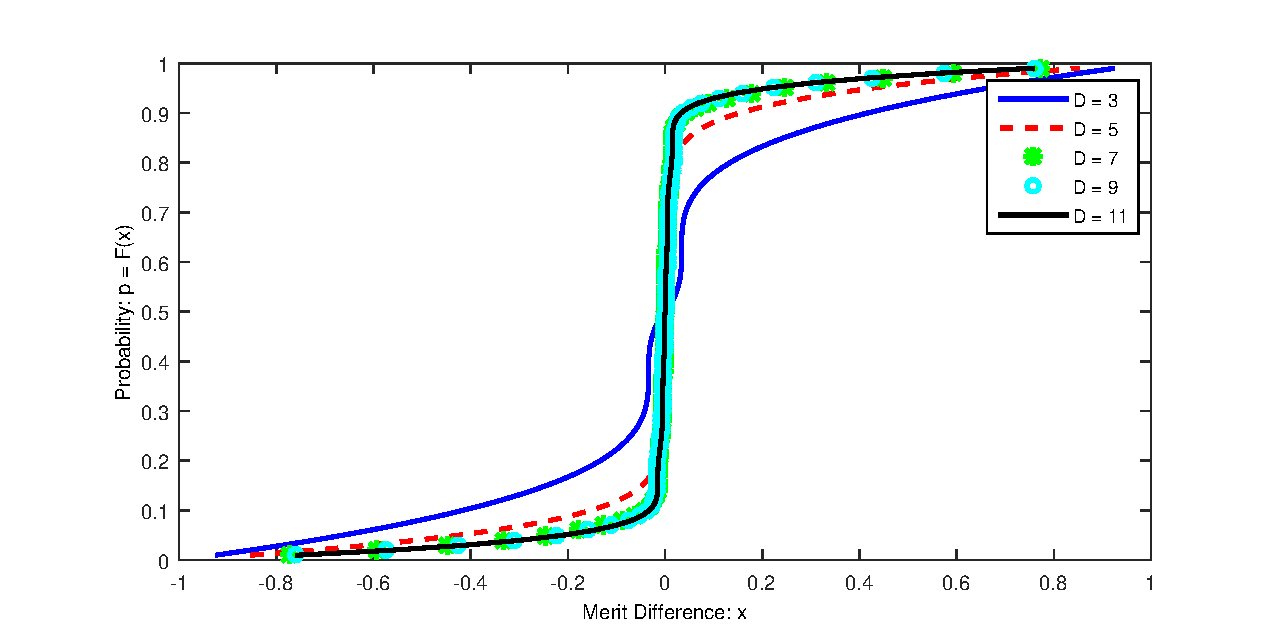
\includegraphics[width=1\textwidth]{chess_more_dimensions.eps}
    \caption{The effect of increasing the dimension $D$ in estimating function $F$. \label{fig:chess_more_dimensions}}
\end{figure}

\begin{figure}
  \centering
    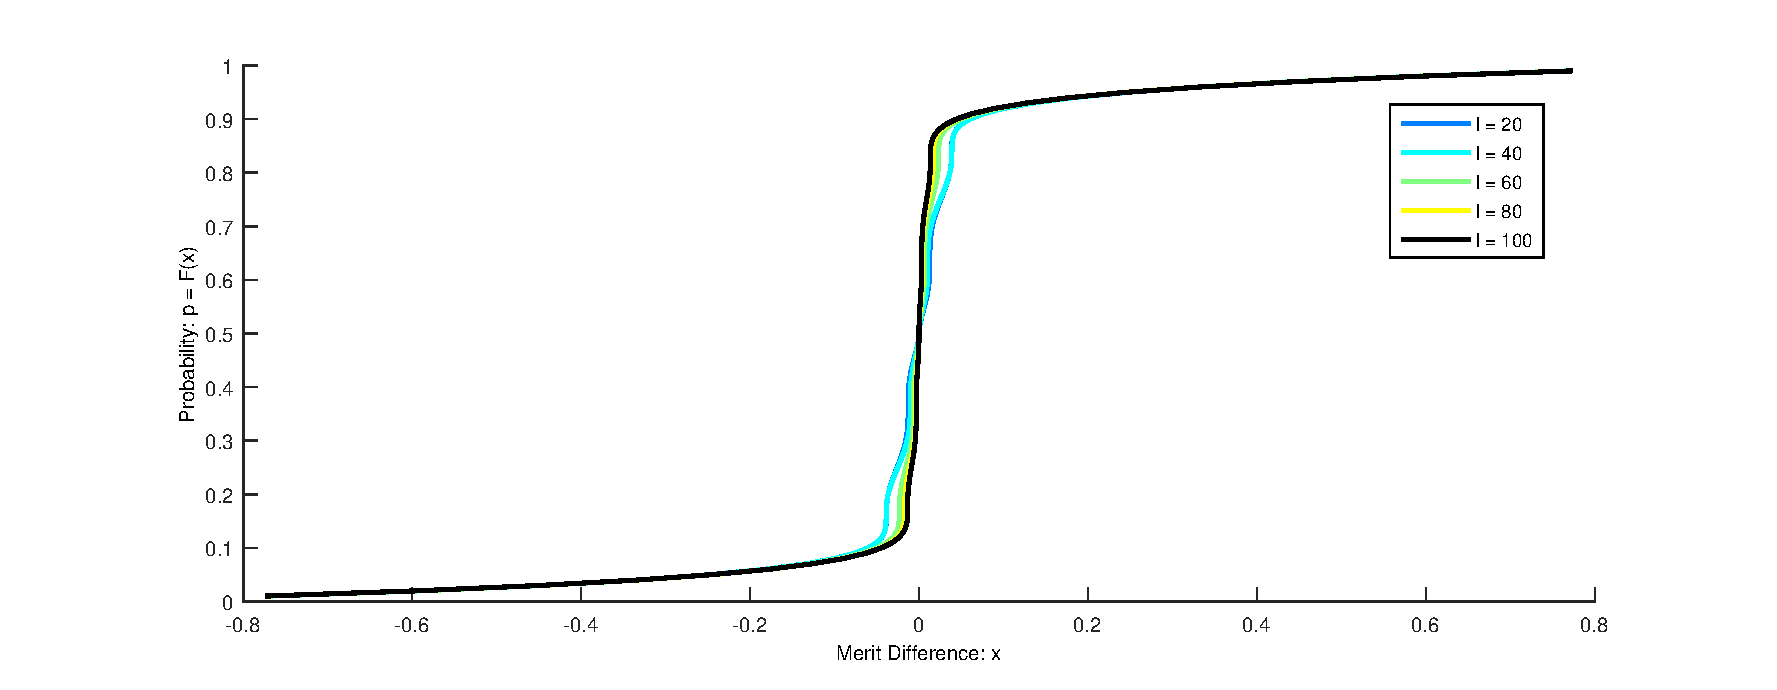
\includegraphics[width=1\textwidth]{chess_more_data.eps}
    \caption{The effect of increasing the amount of data in estimating function $F$. \label{fig:chess_more_data}}
\end{figure}

\begin{figure}
  \centering
    \includegraphics[width=1\textwidth]{PolyRank_vs_BTL_models.eps}
    \caption{Bradley-Terry-Luce models compared to the best fit comparison function. \label{fig:polyrank_vs_BTL}}
\end{figure}

To illustrate this point consider three players $i,j$ and $k$ such that $p_{ij} = p_{jk} = \alpha>0.5$ and $p_{ik} = \beta$, then, from (\ref{eq:linear_model}) we have that $\beta = F(2F^{-1}( \alpha))$. For low values of $ \alpha$ (say $ \alpha = 0.55$) the BTL model and the polynomila model estimated by \textsc{PolyRank} virtually agree on the value of $\beta$ (BTL: $\beta \approx 0.6$; Polynomial: $\beta \approx 0.59$); for intermediate values of $\alpha$ (say, $\alpha = 0.7$) the models begin to diverge $\beta\approx 0.84$; Polynomial: $\beta\approx 0.77$) and for large values of $ \alpha$ (say $ \alpha = 0.9$) this divergence is even more extreme (BTL: $\beta\approx 0.99$; Polynomial: $\beta\approx 0.92$). The estimated polynomial model seems to be more agreeable with the the data at hand since very few chess engines had a (near) perfect win against any opponent.  It will be interesting to investigate whether our findings hold for human chess as well.

\newpage
\section{Summary and Discussion}
\label{sec:discussions}

In this paper we propose a new method for analyzing paired comparison data. Our main contribution is to relax the assumption that the comparison function is known in advance. Instead, we assume that the inverse of the comparison function is a $D$'th degree polynomial and the comparison function has a bounded support. We show that estimation reduces to a tractable SDP that simultaneously recovers the merit vector and the underlying comparison function $F$ from  an initial estimator $\boldsymbol{\hat P}$. We refer to this new methodology as \textsc{PolyRank}. We provide non-stochastic as well as stochastic guarantees for our estimators. This includes a thorough sensitivity analysis and additionally convergence and concentration bounds. Our simulation study demonstrates that the method works well in practice. Finally, we investigate a large data set of computer chess matches and provide evidence that the comparison function used for calculating chess ratings for almost nine decades seems to be inadequate, at least for computer chess engines.

Our work shows that \textsc{PolyRank} can be used whenever the existing methods, which assume that the comparison function is known, are used. The only additional requirement is that the comparison graph must have at least $I+D-1$ edges, a condition which is almost always satisfied in practice. Thus, \textsc{PolyRank} provides a flexible and principled alternative to the existing methods for ranking and rating which are based on paired comparisons. Our analysis, however, is just a starting point and many open research problems remain. It is clear that \textsc{PolyRank} can be extended in various directions; these can be grouped into several domains including: $(i)$ modelling issues; $(ii)$ computational/numerical issues; $(iii)$ statistical and inferential problems of varied types. \\
\\
\textit{Modelling.} We have assumed that $F^{-1}$ is given by a polynomial. Many other models, in which the polynomial in (\ref{eq:F_inv}) is replaced by some other set of basis functions, are possible. Monotone splines provide a class of such functions \citep{ramsay}. One other interesting possibility, with more of a statistical flavor, is to write 
\begin{equation*}
    F^{-1}(p)= \sum_{i = 1}^{D} \beta_i K_i(p)
 \end{equation*}% remark.. notice that "E[F^-1(p)] ~= (E(F(x))^-1", so Im not sure what can be said of the mixture model model function
where $K_i(p)$ are themselves quantile functions of symmetric random variables. This equation can be viewed as a mixture model on the quantile scale. The family $\{K_i\}$ is then chosen by the investigator; the symmetrized beta family of distributions seems like a suitable family to explore. Another, important issue is the incorporation of covariates, such as time or a ``home advantage", as well as many others in the model. This, again, can be done in several ways. The merits can be modeled as regression functions or alternatively one can incorporate the covariates directly into the comparison function. Other issues which deserve attention are the modelling of ties and the comparison of more than two items a time. \\
\\
\textit{Computations and Numerics.} Compared with traditional methods, where the comparison function is given, \textsc{PolyRank} has higher computational complexity and may suffer from numerical instability. In part, the numerical issues are related to our decision to model the inverse of the comparison function as a polynomial. This in turn entails that the normal equations are associated with Vandermonde matrices. A known way to circumvent this problem is to use a different basis for solving equation (\ref{eq:linear_equation}), this amounts to choosing a different  basis for the polynomial regression, such as Chebyshev Polynomials. Another possibility is the use of a different loss function which is less sensitive to numerical issues. Developing a method to uncouple the estimation of $F$ and of $\boldsymbol{\mu}$ as we provided for the unweighted $\mathcal{L}_2$ norm might provide further insight in this direction.
One other, future objective, is to extend the practical reach of \textsc{PolyRank} to larger values of $D$ and $I$ while at the same time increasing computational and numerical efficiency. There may be several ways of doing so. One approach is hand crafting a solver for the SDP at hand. Another possibility is developing an online distributed version of \textsc{PolyRank} in which the function and the merits are updated after each pairwise comparison is observed. \\
\\
\textit{Statistics.} The current paper leaves many statistical issues unresolved. For example, we did not provide any results on the asymptotic distributions of our estimated parameters. We believe, however, that normal limits are obtained provided $(\boldsymbol{\mu},\boldsymbol{\beta})$ are in the interior of the parameter space. It is also clear that employing the one step method we can obtain a fully efficient estimator \citep{fan}.  Other issues of interest are limit theorems for the case where $I \to \infty$ and when paired comparisons are made adaptively. In the adaptive set up one may exploit the fact that function $F$ can be recovered up to arbitrary precision by using a small subset of the items in order to reduce the overall query complexity of the paired comparison experiment.


%for example, one could investigate the induced distribution of the parameters estimated by \textsc{PolyRank}. Concerning model selection, one may define the loss function on the probability space instead of the quantile space, or even test the hypothesis that the residual in (\ref{prob:semi_param_estimation}) is zero for the chosen value of $D$. % Our numerical experiments show that our refined estimators seem to be biased and it remains an open question whether it is possible to devise a refinement procedure that is both computable in polynomial time and unbiased.
%Of coarse, our use of quantile functions is motivated by the fact that directly minimizing $ ||F(\Delta \boldsymbol{\mu}) - \boldsymbol{\hat{P}}||$ or maximizing the likelihood leads to highly intractable computational problems. One possibility is to investigate the one step procedure \citep{fan} to further refine \textsc{PolyRank} and ensure asymptotic efficiency.  Finally,  


%the archetypal problem in contest theory,   one archetypal problem is to, given the number of soldiers in a battle, estimate the chances that one side will win. One could extend \textsc{PolyRank} by using a monotonic relation  $\mu_i = g(x_i)$  where $x_i$ is the number of soldiers and $g$ is monotonic function. If one estimates $g$ as a monotone polynomial as well as the comparison function one could show that the overall problem remains a tractable convex optimization problem.

%\begin{enumerate}
    
%    \item Alternatives and extensions to \textsc{PolyRank}:
%        \subitem Our use of quantile functions is motivated by the fact that directly minimizing $ ||F(\Delta \boldsymbol{\mu}) - \boldsymbol{\hat{P}}||$ or maximizing the likelihood leads to highly intractable computational problems. One possibility is to further refine our estimators with the one step procedure \citep{fan} which can guarantee asymptotic efficiency.
        %\subitem We may generalize our estimation procedure to functional estimation given monotonic relations $\hat{\delta}_{ij}$ that are monotonically related to the difference between the merits $\mu_i-\mu_j$ with an unknown relation $g(\delta_{ij}) = \mu_i-\mu_j$.
%        \subitem In the contest theory, one archetypal problem is: given the number of soldiers in a battle what are the chances that each side will win the fight? One could extend \textsc{PolyRank} by adding a relation  $\mu_i = g(x_i)$  where $x_i$ is the number of soldiers and $g$ is monotonic function. If one estimates $g$ as well as the parameters in \textsc{PolyRank} one could show that the overall problem remains a convex optimization problem with tractable solution.
%        \subitem In so many settings, such as  chess, ties are not only a possible outcome of a paired comparison but a prevalent one. In other settings, such as online games, the comparisons are not done in a pairwise fashion. One challenge is to extend \textsc{PolyRank} to incorporate these possibilities.
        
%    \item Statistical Issues:
%        \subitem Concerning the distribution of the estimated parameters we know very little, e.g., does our estimation procedure induce a  Gaussian distribution on the estimators? 
%        \subitem We have barely scratched the surface of model selection criterion. Why not define the loss function on the probability space instead of the quantile space? Or why not choose the first $D$ such that a test for  $||F^{-1}(\boldsymbol{P})-\Delta\boldsymbol{\mu} ||= 0$ returns a positive answer?    
%        \subitem Our numerical experiments show that the estimators refined by \textsc{PolyRank} are biased. It remains an open question whether it is possible to devise a refinement procedure that is both computable in polynomial time and is unbiased.
        
%    \item Query Complexity:
%        \subitem One could exploit the fact that function $F$ can be recovered up to arbitrary precision and return to the use of the LS method. Could this lead to a reduction of query complexity?
%        \subitem We considered $m_{ij}$ to be fixed. When the  comparisons are chosen adaptively one typically finds a significant reduction in the query complexity. 
        
%    \item Computational Issues:
%        \subitem We have provided a reduction of the general SDP to a smaller one when the weights are equal. We believe it may be possible to develop a similar methodology for the general weights.
%        \subitem We have been handling the reduced SDP problem with a general solver. Could a handcrafted solver exploit the structure of the smaller SDP?
%        \subitem In several contexts an online distributed version of \textsc{PolyRank} may be of interest. For example one could develop a new version of Elo's rating making use of similar mechanics developed for \textsc{PolyRank}. 
        
%    \item Simulations and Real Data:
%        \subitem Our findings concerning computer chess matches seem to provide strong evidence against the traditional use of Bradley-Terry-Luce models for the game of chess. Of coarse human chess players, as well as different modalities of chess games, can be expected to have a different comparison functions; our finding can be strengthened if other data-sets were to be investigated.
        
%        \subitem We have noticed in various simulations that the parameter beta converges very slowly, whereas the geometry of F seems to converge fast. this is because two polynomials may be $\epsilon$ close in the Chebyshev distance but their parameters can be exponentially far away.
        
%        \paragraph{Numerical Stability} Notice that our estimation procedure involves the inversion of a (possibly ill-conditioned) matrix and so even with a matrix $\boldsymbol{\hat P}$ estimated with arbitrary precision one might end up with estimators $\hat \beta$ and $\hat \mu$ skewed by the numerical calculations ...
%\end{enumerate} 


\acks This paper was written when the first author was a graduate student at the Israel Institute of Technology. The research leading to these results has received funding from the European Research Council under European Union's Horizon 2020 Program, ERC Grant agreement no. 682203 ``SpeedInfTradeoff" and the research of Ori Davidov was partially supported by the Israeli Science Foundation Grants No. 1256/13 and 457/17.

\newpage
\appendix
\section{Proof of Theorems}
The following contains the proofs of our main results.
\subsection{Proof of Theorem \ref{the:sdp_set}}
\label{sec:proof_sdp_set}
%In order to prove Theorem \ref{the:sdp_set} we provide  two known results on non-negative polynomials \citep{parrilo}:
%\begin{lemma}%[Sum of Squares Polynomials]
%\label{lemma_SOS}
%Let $P(x)$ be a polynomial of degree at most $2d$. Then the following conditions are equivalent:
%\begin{enumerate}
%	\item $P(x) = \sum_{i = 0}^{2d}c_ix^i$ can be written as a sum of squares of polynomials;
%	\item There exists $\boldsymbol{Q}\in S^{d+1}_+$ such that $c_i = \sum_{j+k = i} Q_{jk}$; \end{enumerate}
%\end{lemma}
%\begin{theorem}%[Non-negative Polynomials]
%\label{the:nonnegative_poly}
%Let $P(x)$ be a polynomial of even degree. Then $P(x)$ is non-negative over the interval $[a,b]$ if and only if it can be written as: $P(x) = s(x) + (x-a)(b-x)t(x)$ where $s(x)$ and $t(x)$ are sum of squares polynomials of degree at most $2d$ and $2d-2$ respectively.
%\end{theorem}

\begin{proof} The constraint $F(0) = 1/2$ is equivalent to $F^{-1}(1/2) = \sum_{i = 0}^D \beta_i\left(1/2\right)^i = 0,$
which is  the last equality constraint in (\ref{SDP_characterization}). Also, $F$ is increasing iff $F^{-1}(p)$ is increasing and  for our set of polynomials this is equivalent to $(F^{-1}(p))' = \beta_1+2\cdot \beta_2p + ...+D\cdot \beta_D p^{D-1}\geq 0$ for every $p \in [0,1/2]$. In addition, $F$ is L-Lipschitz continuous and so  $|F'(x)| \leq L$; which combined with the monotonicity constraint is equivalent to the constraint $(F^{-1}(p))' \geq 1/L$. By Theorem 6 of \citep{parrilo} we have that $(F^{-1}(p))' - 1/L = s(x) + x(1/2-x)t(x)$ where $s(x)$ and $t(x)$ are sum of squares polynomial functions of degree at most $2d$ and $2d-2$ respectively. Now by Lemma 4 of \citet{parrilo} there exists $\boldsymbol{Q^0}\in \mathbb{S}_+^{d+1}$ and $\boldsymbol{Q^1}\in \mathbb{S}_+^{d}$ such that the coefficients of the polynomials $s(x)$ and $t(x)$ are $s_i = \sum_{j+k=i}Q^0_{jk}$ and $t_i = \sum_{j+k=i}Q^1_{jk}$. By combining these conditions on the polynomial $(F^{-1}(p))' - 1/L$ and the constraint $||\boldsymbol{\beta}||_{\infty} \leq U$ we obtain the desired result.
 \end{proof}
 
\subsection{Proof of Theorem \ref{the:sensitivity_LS}}
\label{sec:proof_the_sensitivity_LS}
\begin{proof} 
A little algebra show that \begin{equation}
\label{technical_lemma}||\Delta\boldsymbol{\hat \mu} - \Delta\boldsymbol{\mu}||_2^2 = 2n||\boldsymbol{\hat \mu} - \boldsymbol{\mu}||^2_2;\end{equation}
this is so because
$$||\Delta\boldsymbol{\hat \mu} - \Delta\boldsymbol{\mu}||_2^2 = \sum_{ij}(\hat{\mu}_i - \hat{\mu}_j - \mu_i+\mu_j)^2 = 2n||\boldsymbol{\hat \mu} - \boldsymbol{\mu}||^2_2 - 2 ( \sum_{i}\hat{\mu}_i- \sum_i \mu_i )^2$$%\sum_{ij}(\hat{\mu}_i- \mu_i)^2 + (\hat{\mu}_j -\mu_j)^2 - 2\cdot (\hat{\mu}_i- \mu_i)(\hat{\mu}_j -\mu_j)   = $$
%$$=\sum_{ij}(\hat{\mu}_i- \mu_i)^2 + (\hat{\mu}_j -\mu_j)^2 - 2 \sum_{i} \sum_j (\hat{\mu}_i- \mu_i)(\hat{\mu}_j -\mu_j)   = 2n||\boldsymbol{\hat \mu} - \boldsymbol{\mu}||^2_2 - 2 \sum_{i}(\hat{\mu}_i- \mu_i) \sum_j (\hat{\mu}_j -\mu_j) =  $$
%$$= 2n||\boldsymbol{\hat \mu} - \boldsymbol{\mu}||^2_2 - 2 ( \sum_{i}\hat{\mu}_i- \sum_i \mu_i )^2$$
where the last term is zero by construction. It follows that
%Thus, equation (\ref{eq:merit_sens_known}) stems from the fact that
$$||\boldsymbol{\hat \mu}-\boldsymbol{\mu}||_2 = \frac{1}{\sqrt{2n}}||\Delta\boldsymbol{\hat \mu}-\Delta\boldsymbol{\mu}||_2  \leq \frac{1}{\sqrt{2n}}||F^{-1}(\boldsymbol{\hat P})-\Delta\boldsymbol{\mu} ||_2 $$
$$=\frac{1}{\sqrt{2n}}||F^{-1}(\boldsymbol{\hat P})-F^{-1}(\boldsymbol{ P})||_2  \leq \frac{4U}{\sqrt{2n}}||\boldsymbol{\hat P}-\boldsymbol{P}||_2.$$ The first inequality is a conscequence of the convex projection theorem and the first  equality follows from (\ref{technical_lemma}). Equation (\ref{eq:prob_sens_known}) is derived from $$||\boldsymbol{P}^*-\boldsymbol{P}||_2^2 = ||F(\Delta \boldsymbol{\hat{\mu}})-F(\Delta \boldsymbol{\mu})||_2^2 \leq L^2 || \Delta \boldsymbol{\hat \mu} -\Delta \boldsymbol{\mu} ||_2^2 = L^2 2 n||\boldsymbol{\hat \mu} - \boldsymbol{\mu}||_2^2 \leq L^2 (4U)^2||\boldsymbol{\hat P} - \boldsymbol{P}||_2^2.$$ Where the last equality is an application of equation (\ref{technical_lemma}) and the last inequality an application of (\ref{eq:merit_sens_known}). If $\boldsymbol{\hat{P}}$ is assumed to obey strong stochastic transitivity, then  $\hat{p}_{ij}<1/2$ implies that $\hat{p}_{ik}\leq \hat{p}_{jk}$ for all $k$ and $\hat{p}_{ik} < \hat{p}_{jk}$ for at least some $k$. Thus, the identity $\hat{\mu}_i - \hat{\mu}_j = (1/n)\sum_k (F^{-1}(\hat{p}_{ik}) - F^{-1}(\hat{p}_{jk}))<0$ together with the fact that $F^{-1}$ is strictly monotone assures that the strong stochastic transitivity order is the same as the order of the estimated merits.
\end{proof}

\paragraph{Remark} Theorem \ref{the:sensitivity_LS}, applies to other norms with the proper modifications. Assume that the estimator $\boldsymbol{P}^*$ is obtained via (\ref{eq:ls_matrix}) under the norm or semi-norm $||\cdot||_{\#}$. Let $L_{\#}$ and $4U_{\#}$ be the Lipschitz constants of $F$ and $F^{-1}$ associated with $||\cdot||_{\#}$, then 
    
$$||\boldsymbol{P^*} - \boldsymbol{P}||_{\#} \leq ||\boldsymbol{\hat P} - \boldsymbol{P^*}||_{\#}+||\boldsymbol{\hat P} - \boldsymbol{P}||_{\#} \leq L_{\#} ||F^{-1}(\boldsymbol{\hat P}) - \Delta \boldsymbol{\hat{\mu}}||_{\#}+||\boldsymbol{\hat P} - \boldsymbol{P}||_{\#}  \leq$$ $$  L_{\#} ||F^{-1}(\boldsymbol{\hat P}) - \Delta \boldsymbol{\mu}||_{\#}+||\boldsymbol{\hat P} - \boldsymbol{P}||_{\#}\leq 4L_{\#}U_{\#}||\boldsymbol{\hat P} - \boldsymbol{P}||_{\#}+ ||\boldsymbol{\hat P} - \boldsymbol{P}||_{\#} = (1+4L_{\#}U_{\#})||\hat{\boldsymbol{P}} - \boldsymbol{P}||_{\#},$$
as in (\ref{eq:prob_sens_known}). 
%
%$L_1$ - norm
%$$|\hat{\mu}_i - \mu_i| = \left|\frac{1}{n} \sum_{j = 1}^nF^{-1}(\hat{p}_{ij}) - \frac{1}{n} \sum_{j = 1}^nF^{-1}(p_{ij})\right| = \left| \frac{1}{n} \sum_{j = 1}^nF^{-1}(\hat{p}_{ij})-F^{-1}(p_{ij}) \right| \leq $$
%$$\leq \frac{1}{n} \sum_{j = 1}^n \left|F^{-1}(\hat{p}_{ij})-F^{-1}(p_{ij}) \right|\leq \frac{1}{n} \sum_{j = 1}^n U\left|\hat{p}_{ij} - p_{ij} \right| =\frac{U}{n} \sum_{j = 1}^n \left|\hat{p}_{ij} - p_{ij} \right| $$
%Therefore summing on  $i$ we get:
%$$ ||\boldsymbol{\hat \mu}  - \boldsymbol{\mu}||_1 \leq \frac{U}{n} \sum_{i = 1}^{n}\sum_{j = 1}^n \left|\hat{p}_{ij} - p_{ij} \right| = \frac{U}{n} ||\boldsymbol{\hat P} - \boldsymbol{P}||_1$$
%$L_{\infty}$ - norm  
% $$||\boldsymbol{\hat \mu} - \boldsymbol{\mu}||_{\infty} = \max_i |\frac{1}{n}\sum_j F^{-1}(\hat{p}_{ij}) -F^{-1}(p_{ij}) | \leq \max_i \frac{1}{n} \sum_j |F^{-1}(\hat{p}_{ij}) - F^{-1}(p_{ij}))| \leq$$
% $$\leq\max_i \frac{U}{n} \sum_j|\hat{p}_{ij} - p_{ij}| \leq \max_i \frac{U}{n} n \max_j|\hat{p}_{ij} - p_{ij}| =U \max_{ij}|\hat{p}_{ij} - p_{ij}|$$\\ \\
%$L_1$ - norm 
%$$||\boldsymbol{P}^*-\boldsymbol{P}||_1 = \sum_{ij} |F(\hat{\mu}_i -\hat{\mu}_j) - F(\mu_i -\mu_j)| \leq L \sum_{ij}|\hat{\mu}_i -\hat{\mu}_j - \mu_i +\mu_j| \leq$$
%$$\leq L \sum_{ij}|\hat{\mu}_i-\mu_i|  +| \hat{\mu}_j - \mu_j| = 2n L ||\boldsymbol{\hat \mu} - \boldsymbol{\mu}||_1 \leq_{[1]} 2 LU ||\boldsymbol{\hat P} - \boldsymbol{P}||_1$$
%[1] By the sensitivity of the merit vector. \\
%$L_{\infty}$ - norm 
%$$||\boldsymbol{\hat P} -\boldsymbol{P}||_{\infty} = \max_{ij}|F(\hat{\mu}_i - \hat{\mu}_j)-F(\mu_i - \mu_j)| \leq L \max_{ij} |\mu_i - \mu_j -\hat{\mu}_i - \hat{\mu}_j| \leq L \max_{ij} |\hat{\mu}_i-\mu_i| + | \hat{\mu}_j-\mu_j | =$$
%$$ = 2 L \max_i |\hat{\mu}_i-\mu_i|= 2 L ||\boldsymbol{\hat \mu} -\boldsymbol{\mu}||_{\infty} \leq_{[1]} 2 LU||\boldsymbol{\hat P} - \boldsymbol{P}||_{\infty}$$
%[1] By the sensitivity of the merit vector.\\


\subsection{Proof of Theorem \ref{the:sensitivity_realizable}}
\label{sec:proof_the_sensitivity_realizable}

\begin{proof} %First notice that for every function  $F_{\boldsymbol{\beta}}\in \mathcal{F}$, the inverse $F^{-1}_{\boldsymbol{\beta}}$ is $4U$-Lipshitz continuous. This is true because by the mean value theorem we have that $F^{-1}_{\boldsymbol{\beta}}(a) - F^{-1}_{\boldsymbol{\beta}}(b) = ( a - b) \left(F^{-1}_{\boldsymbol{\beta}}\right)'(c)$ for some $c$ in the interval betweeb $a$ and $b$, therefore we have that $\left|F^{-1}_{\boldsymbol{\beta}}(a) - F^{-1}_{\boldsymbol{\beta}}(b)\right| = \left|a - b\right|  \left|\left(F^{-1}_{\boldsymbol{\beta}}\right)'(c) \right| \leq \left|a - b\right|  \max_{p \in [0,1]}\left|\left(F^{-1}_{\boldsymbol{\beta}}\right)'(p)\right|.$
%Notice though that from the equation $F_{\boldsymbol{\beta}}(x)+F_{\boldsymbol{\beta}}(-x) = 1$ we have that $F_{\boldsymbol{\beta}}^{-1}(p) + F_{\boldsymbol{\beta}}^{-1}(1-p) = 0$
%and therefore
%$\left(F_{\boldsymbol{\beta}}^{-1}\right)'(p) = \left(F_{\boldsymbol{\beta}}^{-1}\right)'(1-p) $
%and so we find that 
%$$\max_{p \in [0,1]}\left|\left(F^{-1}_{\boldsymbol{\beta}}\right)'(p)\right| = \max_{p \in [0,1/2]}\left|\left(F^{-1}_{\boldsymbol{\beta}}\right)'(p)\right|$$
%now by the definition of $\mathcal{F}$, for $p\in[0,1/2]$, we have  $\left|\left(F^{-1}_{\boldsymbol{\beta}}\right)'(p)\right| = \left|\beta_1 + 2\beta_2 p +...+D\beta_Dp^{D-1}\right|$; and so
%$\max_{p \in [0,1/2]}\left|\left(F^{-1}_{\boldsymbol{\beta}}\right)'(p)\right| = \max_{p \in [0,1/2]}\left|\beta_1 + 2\beta_2 p +...+D\beta_Dp^{D-1}\right| \leq \max_{p \in [0,1/2]}\left|\beta_1\right| + \left|2\beta_2 p\right| +...+\left|D\beta_Dp^{D-1}\right| \leq \max_{p \in [0,1/2]} \left(\max_{i = 0,...,D} |\beta_i|\right) \cdot \left(1 + \left|2p\right| +...+\left|Dp^{D-1}\right|\right);$ this can be further simplified to 
%$  ||\boldsymbol{\beta}||_{\infty} \cdot (1 + 2\cdot\left(\frac{1}{2}\right) +...+D\left(\frac{1}{2}\right)^{D-1}) \leq 4U .$
%The $D'$th partial sum of a geometric series with ratio $r\neq 1$ is:
%$$1+r+...+r^D = \frac{1-r^{D+1}}{1-r}$$
%deriving this equation we have
%$$1+2r+...+Dr^{D-1} = \left(\frac{1-r^{D+1}}{1-r}\right)' = \frac{1-r^{D+1} - (D+1)r^D(1-r)}{(1-r)^2} = \frac{1-r^{D} \left[r +(D+1)(1-r) \right]}{(1-r)^2}$$
%substituting $r=1/2$ we have
%$$\left(1 + 2\cdot\left(\frac{1}{2}\right) +...+D\left(\frac{1}{2}\right)^{D-1}\right) = \frac{1-(\frac{1}{2})^{D} \left[\frac{1}{2} +(D+1)(1-(\frac{1}{2})) \right]}{(1-(\frac{1}{2}))^2} = 4 - (1/2)^{D-1}(D+2) \leq 4$$
%We may now progressively prove our results:
%1. Empirical Loss:
%$$\left| \left| F^{-1}_{\boldsymbol{\hat \beta }}(\boldsymbol{\hat{P}}) - \Delta \boldsymbol{\hat \mu} \right| \right| \leq_{[1]} \left| \left| F^{-1}_{\boldsymbol{\beta}}(\boldsymbol{\hat{P}}) - \Delta \boldsymbol{\mu} \right| \right|  \leq_{[2]} \left| \left| F^{-1}_{\boldsymbol{\beta}}(\boldsymbol{P}) - \Delta \boldsymbol{\mu} \right| \right| + 4U||\boldsymbol{\hat{P}} - \boldsymbol{P}|| =_{[3]} 4U||\boldsymbol{\hat{P}} - \boldsymbol{P}|| $$
%[1] By the optimality of $\boldsymbol{\hat \beta}$ and $\boldsymbol{\hat \mu}$.
%[2] By Lemma \ref{lemma:lipschitz}.
%[3] By realizability of the underlying model.\\
%2. True Loss:
%$$\left| \left| F^{-1}_{\boldsymbol{\hat{\beta}}}(\boldsymbol{P}) - \Delta \boldsymbol{\hat{\mu}} \right| \right| \leq_{[1]} \left| \left| F^{-1}_{\boldsymbol{\hat{\beta}}}(\boldsymbol{\hat{P}}) - \Delta \boldsymbol{\hat{\mu}} \right| \right|  +4U||\boldsymbol{\hat{P}} - \boldsymbol{P}||\leq_{[2]} 4U||\boldsymbol{\hat{P}} - \boldsymbol{P}||+4U||\boldsymbol{\hat{P}} - \boldsymbol{P}|| $$
%[1] By Lemma \ref{lemma:lipschitz}.
%[2] By the empirical risk sensitivity bound.\\
%3. Probability Matrix Sensitivity:\\
%By the true risk sensitivity bound we have that
%$$F^{-1}_{\boldsymbol{\hat{\beta}}}(\boldsymbol{P}) = \Delta \boldsymbol{\hat{\mu}} + \boldsymbol{\zeta} $$
%where $|| \boldsymbol{\zeta} || \leq 8U||\boldsymbol{\hat{P}} - \boldsymbol{P}||$ and therefore 
%$$||\boldsymbol{P^*} - \boldsymbol{P}||  = \left| \left| F_{\boldsymbol{\hat{\beta}}}\left( F^{-1}_{\boldsymbol{\hat{\beta}}}(\boldsymbol{P})\right) - F_{\boldsymbol{\hat{\beta}}}\left( \Delta \boldsymbol{\hat{\mu}}\right) \right| \right| = \left| \left| F_{\boldsymbol{\hat{\beta}}}\left(\Delta \boldsymbol{\hat{\mu}} + \boldsymbol{\zeta}\right) - F_{\boldsymbol{\hat{\beta}}}\left( \Delta \boldsymbol{\hat{\mu}}\right) \right| \right|  $$
%$$\therefore ||\boldsymbol{P^*} - \boldsymbol{P}|| \leq L ||\boldsymbol{\zeta}|| \leq 8LU||\boldsymbol{\hat{P}} - \boldsymbol{P}||$$
Equation (\ref{eq:sensitivity_realizable}) is a conscequence of
$$||\boldsymbol{P^*} - \boldsymbol{P}|| \leq ||\boldsymbol{\hat P} - \boldsymbol{P^*}||+||\boldsymbol{\hat P} - \boldsymbol{P}|| \leq L ||F^{-1}_{\boldsymbol{\hat \beta}}(\boldsymbol{\hat P}) - \Delta \boldsymbol{\hat{\mu}}||+||\boldsymbol{\hat P} - \boldsymbol{P}||  $$ $$ \leq L ||F^{-1}_{\boldsymbol{ \beta}}(\boldsymbol{\hat P}) - \Delta \boldsymbol{\mu}||+||\boldsymbol{\hat P} - \boldsymbol{P}||\leq 4LU||\boldsymbol{\hat P} - \boldsymbol{P}||+ ||\boldsymbol{\hat P} - \boldsymbol{P}||;$$
where the last inequality stems from the fact that $F^{-1}_{\boldsymbol{ \beta}}(p)$ is $4U$-Lipschitz continuous  for every $F_{\boldsymbol{ \beta}}(p) \in \mathcal{F}$ and the previous inequality is a consequence of the optimality of \textsc{PolyRank}. In order to prove (\ref{eq:parameter_sensitivity}), consider a set of linear equations $\boldsymbol{A} \boldsymbol{x} = \boldsymbol{b}$ and a perturbed version $(\boldsymbol{A}+\Delta \boldsymbol{A})(\boldsymbol{x}+\Delta \boldsymbol{x}) = b$ where both $\boldsymbol{A}$ and $\boldsymbol{A}+\Delta \boldsymbol{A}$ are non-singular square matrices. Under these conditions one can show that $\Delta \boldsymbol{x} = \boldsymbol{A}^{-1}\Delta \boldsymbol{A}(\boldsymbol{x}+\Delta \boldsymbol{x})$; %this is so because
%$$\Delta x = (A + \Delta A)^{-1} b - A^{-1}b = A^{-1}(A(A+\Delta A)^{-1}-I)b = $$
%$$= A^{-1}(A(A+\Delta A)^{-1}-I)(A+\Delta A)(x+\Delta x) = A^{-1}(A-A+\Delta A)(x+\Delta x) = $$
%$$= A^{-1}\Delta A(x+\Delta x).$$
thus:%i.e., define $b = \left(\begin{array}{c}
%     -\boldsymbol{\beta}_0 \\
%     0 
%\end{array}\right)$, $A = A(\boldsymbol{P})$, $x = \left(\begin{array}{c}
%     \boldsymbol{\beta} \\
%     \boldsymbol{\mu} 
%\end{array}\right)$, $A+\Delta A = A(\boldsymbol{P^*})$ and $x+\Delta x = \left(\begin{array}{c}
%     \boldsymbol{\hat{\beta}} \\
%     \boldsymbol{\hat{\mu}} 
%\end{array}\right)$; which gives the identity
\begin{equation}
\label{eq:relation}
\left(\begin{array}{c}
     \boldsymbol{\hat{\beta}} -\boldsymbol{\beta}\\
     \boldsymbol{\hat{\mu}} -\boldsymbol{\mu} 
\end{array}\right) = \boldsymbol{A}(\boldsymbol{P})^{-1}[\boldsymbol{A}(\boldsymbol{P^*}) - \boldsymbol{A}(\boldsymbol{P})]\left(\begin{array}{c}
     \boldsymbol{\hat{\beta}} \\
     \boldsymbol{\hat{\mu}} 
\end{array}\right).
\end{equation}
%Therefore:
%$$ \left|\left|\left(\begin{array}{c}
%     \boldsymbol{\hat{\beta}} -\boldsymbol{\beta}\\
%     \boldsymbol{\hat{\mu}} -\boldsymbol{\mu} 
%\end{array}\right) \right|\right| \leq || A(\boldsymbol{P})^{-1}|| ||A(\boldsymbol{P^*}) - A(\boldsymbol{P})||\left|\left|\left(\begin{array}{c}
%     \boldsymbol{\hat{\beta}} \\
%     \boldsymbol{\hat{\mu}} 
%\end{array}\right) \right|\right|.$$
Notice  that $||\boldsymbol{\hat{\beta}}||_{\infty} \leq U$ and also  $||\boldsymbol{\hat{\mu}}||_{\infty} \leq U$. The second claim is true for if  $\hat{\mu}_j \geq U$ for some $j$ then $|\hat{\mu}_i -\hat{\mu}_j|= |F_{\boldsymbol{\hat \beta}}^{-1}(\hat{p}_{ij}^*)| \leq |F_{\boldsymbol{\hat \beta}}^{-1}(0)| = |\beta_0| \leq U $ which then implies that $\hat{\mu}_i\geq 0$ for every $i$ and so $\sum_i \hat{\mu}_i \geq U >0$ which violates the constraint $\sum_i \hat{\mu}_i = 0$; therefore we must have $\hat{\mu}_j < U$ for every j (the analogous argument is valid for $\hat{\mu}_j > -U$). Using the equivalence between norms find:

$$\left|\left|\left(\begin{array}{c}
     \boldsymbol{\hat{\beta}} -\boldsymbol{\beta}\\
     \boldsymbol{\hat{\mu}} -\boldsymbol{\mu} 
\end{array}\right) \right|\right| \leq  U\sqrt{I+D} || \boldsymbol{A}(\boldsymbol{P})^{-1}|| ||\boldsymbol{A}(\boldsymbol{P^*}) - \boldsymbol{A}(\boldsymbol{P})||. $$
Now notice that
$$||\boldsymbol{A}(\boldsymbol{P^*}) - \boldsymbol{A}(\boldsymbol{P}) ||^2 = \sum_{k = 1}^{D+I-1}\sum_{n = 1}^{D}(p^{*n}_{(ij)_k}-p^{n}_{(ij)_k})^2 \leq \sum_{k = 1}^{D+I-1}D (p^{*}_{(ij)_k}-p_{(ij)_k})^2 \leq D ||\boldsymbol{P^*} - \boldsymbol{P} ||^2$$
and therefore:
$$\left|\left|\left(\begin{array}{c}
     \boldsymbol{\hat{\beta}} -\boldsymbol{\beta}\\
     \boldsymbol{\hat{\mu}} -\boldsymbol{\mu} 
\end{array}\right) \right|\right| \leq  U(4LU+1)\sqrt{D(I+D)} || \boldsymbol{A}(\boldsymbol{P})^{-1}|| ||\boldsymbol{\hat P} - \boldsymbol{P}||, $$
 which completes the proof of (\ref{eq:parameter_sensitivity}). Now we will prove equation (\ref{eq:chebyshev_convergence}). A bit of algebra shows that for every $F_{\boldsymbol{\beta}} \in \mathcal{F}$ we have that $\max_{\alpha \in [0,1] }|F^{-1}_{\boldsymbol{\beta}}(\alpha) - F^{-1}_{\boldsymbol{\hat \beta}}(\alpha)| \leq 2||\boldsymbol{\hat{\beta}}-\boldsymbol{\beta}||_{\infty}$; 
 %$\max_{\alpha \in [0,1] }|F^{-1}_{\boldsymbol{\beta}}(\alpha) - F^{-1}_{\boldsymbol{\hat \beta}}(\alpha)| = \max_{\alpha \in [0,1/2] }|F^{-1}_{\boldsymbol{\beta}}(\alpha) - F^{-1}_{\boldsymbol{\hat \beta}}(\alpha)|= |F^{-1}_{\boldsymbol{\beta}}(\alpha^*) - F^{-1}_{\boldsymbol{\hat \beta}}(\alpha^*)|  = |\sum_i (\hat{\beta}_i - \beta_i)\alpha^{*i} | \leq \sum_i |\hat{\beta}_i - \beta_i|\alpha^{*i} \leq \left(\max_{i}|\hat{\beta}_i - \beta_i|\right) \cdot (1+\alpha^* + ...+\alpha^{*D})= ||\boldsymbol{\hat{\beta}}-\boldsymbol{\beta}||_{\infty} \left(\frac{1 - \alpha^{*D}}{1-\alpha^*} \right) \leq ||\boldsymbol{\hat{\beta}}-\boldsymbol{\beta}||_{\infty} \left(\frac{1 - (1/2)^{D}}{1-(1/2)} \right) \leq  2||\boldsymbol{\hat{\beta}}-\boldsymbol{\beta}||_{\infty}$
%and therefore $\max_{\alpha  }|F_{\boldsymbol{\hat \beta}}(\alpha) - F_{\boldsymbol{\beta}}(\alpha)|  = \max_{\alpha  }|F_{\boldsymbol{\beta}}(F^{-1}_{\boldsymbol{\beta}}(F_{\boldsymbol{\hat \beta}}(\alpha))) - F_{\boldsymbol{\beta}}(\alpha)| \leq  \max_{\alpha  } L |F^{-1}_{\boldsymbol{\beta}}(F_{\boldsymbol{\hat \beta}}(\alpha)) -\alpha| =  L \max_{\alpha  } |F^{-1}_{\boldsymbol{\beta}}(F_{\boldsymbol{\hat \beta}}(\alpha)) -F^{-1}_{\boldsymbol{\hat \beta}}(F_{\boldsymbol{\hat \beta}}(\alpha))|;$ taking $\alpha' = F_{\boldsymbol{\hat \beta}}(\alpha)$ we have
%$ L \max_{\alpha' \in [0,1] } |F^{-1}_{\boldsymbol{\beta}}(\alpha') -F^{-1}_{\boldsymbol{\hat \beta}}(\alpha')|  \leq 2 L ||\boldsymbol{\beta}-\boldsymbol{\hat{\beta}}||_{\infty}$;
combining this with (\ref{eq:relation}), (\ref{eq:parameter_sensitivity}) and the lipschitz continuity of $F_{\boldsymbol{\beta}}$ we find the desired result. Finally, to prove order preservation, recognize that problem (\ref{SDP_characterization}) can be solved by minimizing in $\boldsymbol{\mu}$ and in $\boldsymbol{\beta}$  separately. By minimizing on $\boldsymbol{\mu}$ we find the same closed form solution as the least squares refinement procedure, namely $\mu_i = (1/I)\sum_j F_{\boldsymbol{\beta}}^{-1}(\hat{p}_{ij})$. The proof follows by the same arguments as in Theorem \ref{the:sensitivity_LS}.
\end{proof}



\subsection{Proof of Theorem \ref{the:underfit}}
\label{sec:proof_the_underfit}

\begin{proof}
We will first prove that $\max_{\alpha \in [0,1] }|F^{-1}_{\boldsymbol{\hat \beta}}(\alpha) - F^{-1}_{\boldsymbol{\beta}}(\alpha)|\geq 2 |\beta_{D}|/8^D$. In the following proof $\mathcal{P}_{D-1}$ is the set of polynomials of degree less than or equal to $D-1$. 
$$\max_{\alpha \in [0,1] }|F^{-1}_{\boldsymbol{\hat \beta}}(\alpha) - F^{-1}_{\boldsymbol{\beta}}(\alpha)| = \max_{\alpha \in [0,1/2] }|F^{-1}_{\boldsymbol{\hat \beta}}(\alpha) - F^{-1}_{\boldsymbol{\beta}}(\alpha)|   $$

$$\geq \min_{G \in \mathcal{F}_{D'}}\max_{\alpha \in [0,1/2] }|G(\alpha) - F^{-1}_{\boldsymbol{\beta}}(\alpha)| \geq \min_{G^{-1} \in \mathcal{P}_{D-1}}\max_{\alpha \in [0,1/2] }|G^{-1}(\alpha) - F^{-1}_{\boldsymbol{\beta}}(\alpha)|  $$
 
$$ = \min_{\begin{array}{c}
     F^{-1}_{\boldsymbol{\tilde{\beta}}} \in \mathcal{P}_{D-1}\end{array} }\max_{\alpha \in [0,1/2] }|F_{\boldsymbol{\tilde{\beta}}}^{-1}(\alpha) +\beta_D\alpha^D| $$

$$=|\beta_D| \min_{\begin{array}{c}
     F^{-1}_{\boldsymbol{\tilde{\beta}}} \in \mathcal{P}_{D-1}\end{array} }\max_{\alpha \in [0,1/2] }|F_{\boldsymbol{\tilde{\beta}}}^{-1}(\alpha)+\alpha^D | $$

$$=|\beta_D| \min_{\begin{array}{c}
     F^{-1}_{\boldsymbol{\tilde{\beta}}} \in \mathcal{P}_{D-1} \end{array} }\max_{\alpha \in [-1,1] }|F_{\boldsymbol{\tilde{\beta}}}^{-1}((\alpha+1)/4)  + ((\alpha+1)/4)^D|$$
     

$$\geq \frac{|\beta_D|}{4^D} \min_{\begin{array}{c}
     F^{-1}_{\boldsymbol{\tilde{\beta}}} \in \mathcal{P}_{D-1} \end{array} }\max_{\alpha \in [-1,1] }|F_{\boldsymbol{\tilde{\beta}}}^{-1}(\alpha) + \alpha^D|  $$

$$ = \frac{|\beta_D|}{4^D}  \frac{1}{2^{D-1}} $$

The last equality is a defining property of Chebyshev polynomials \citep{mason}. Now,  notice that the $4U$-Lipschitz continuity of $F_{\boldsymbol{\beta}}^{-1} $ is equivalent to $|F_{\boldsymbol{\beta}}(y) - F_{\boldsymbol{\beta}}(x)| \geq  (1/4U) |y-x|$; combining this with $\max_{\alpha \in [0,1] }|F^{-1}_{\boldsymbol{\hat \beta}}(\alpha) - F^{-1}_{\boldsymbol{\beta}}(\alpha)|\geq 2 |\beta_{D}|/8^D$ we obtain equation (\ref{eq:chebyshev_bad}).
%$$|F^{-1}_{\boldsymbol{ \beta}}(\theta) - F^{-1}_{\boldsymbol{ \beta}}(\phi) | \leq 4U |\theta - \phi| = 4U |F_{\boldsymbol{\beta}}(F^{-1}_{\boldsymbol{ \beta}}(\theta)) - F_{\boldsymbol{\beta}}(F^{-1}_{\boldsymbol{ \beta}}(\phi))|$$
%and so naming $y=F^{-1}_{\boldsymbol{ \beta}}(\theta)$ and $x =F^{-1}_{\boldsymbol{ \beta}}(\phi)$ we have shown that:
%$$|F_{\boldsymbol{\beta}}(y) - F_{\boldsymbol{\beta}}(x)| \geq \frac{1}{4U} |F^{-1}_{\boldsymbol{ \beta}}(F_{\boldsymbol{\beta}}(y)) - F^{-1}_{\boldsymbol{ \beta}}(F_{\boldsymbol{\beta}}(x))| = \frac{1}{4U} |y-x|$$
%therefore
%$$\max_{\alpha} |F_{\boldsymbol{\hat \beta}}(\alpha) - F_{\boldsymbol{\beta}}(\alpha)| = \max_{\alpha} |F_{\boldsymbol{\beta}}\left( F_{\boldsymbol{\beta}}^{-1} \left(F_{\boldsymbol{\hat \beta}}(\alpha)\right)\right) - F_{\boldsymbol{\beta}}(\alpha)| \geq$$
%$$\geq \max_{\alpha}\frac{1}{\mathcal{L}_{\boldsymbol{\beta}}} |F_{\boldsymbol{\beta}}^{-1} \left(F_{\boldsymbol{\hat \beta}}(\alpha)\right)-\alpha|  = \frac{1}{\mathcal{L}_{\boldsymbol{\beta}}} \max_{\alpha} |F_{\boldsymbol{\beta}}^{-1} \left(F_{\boldsymbol{\hat \beta}}(\alpha)\right)-F_{\boldsymbol{\hat \beta}}^{-1} ( F_{\boldsymbol{\hat \beta}} (\alpha))| = $$
%taking $\alpha' = F_{\boldsymbol{\hat \beta}}(\alpha)$ we have
%$$= \frac{1}{\mathcal{L}_{\boldsymbol{\beta}}} \max_{\alpha' \in [0,1]} |F_{\boldsymbol{\beta}}^{-1} \left(\alpha'\right)-F_{\boldsymbol{\hat \beta}}^{-1} (\alpha')| \geq 2 \frac{|\beta_{D}|}{8^D}$$
\end{proof}

\subsection{Proof of Theorem \ref{the:analytic_sensitivity_LS}}
\begin{proof} Let $\hat{l}(D)$ be the empirical loss of a $D$ dimensional fit provided by \textsc{PolyRank}, then:
$$\hat{l}(D) = \min_{ \beta\in \mathbb{R}^D,    \mu\in\mathbb{R}^{I} } \sqrt{\sum_{(ij)\in \mathcal{S}}(\beta_0+...+\beta_D\hat{p}_{ij}^D - \mu_i +\mu_j)^2 }$$
where  the minimum is taken over the sets specified by  \textsc{PolyRank} for some triplet $(D,U,L)$. It is also true that: 
$$\hat{l}(D) = \min_{ \beta\in \mathbb{R}^{D+1},    \mu\in\mathbb{R}^{I} } \sqrt{\sum_{(ij)\in \mathcal{S}}(\beta_0+...+\beta_D\hat{p}_{ij}^D - \mu_i +\mu_j)^2 }$$
for the set specified by the triplet $(D+1,U,L)$, and so
$$\hat{l}(D) \leq  \min_{\beta\in \mathbb{R}^{D+1}, \mu\in \mathbb{R}^I} \sqrt{\sum_{(ij)\in \mathcal{S}}(\beta_0+...+\beta_D\hat{p}_{ij}^D +\beta_{D+1}\hat{p}_{ij}^{D+1} - \mu_i +\mu_j)^2 }  + \sqrt{\sum_{(ij)\in \mathcal{S}}(\beta_{D+1}\hat{p}_{ij}^{D+1})^2 } $$

$$\leq  \min_{\beta\in \mathbb{R}^{D+1}, \mu\in \mathbb{R}^I} \sqrt{\sum_{(ij)\in \mathcal{S}}(\beta_0+...+\beta_D\hat{p}_{ij}^D +\beta_{D+1}\hat{p}_{ij}^{D+1} - \mu_i +\mu_j)^2 }  + U\sqrt{\sum_{(ij)\in \mathcal{S}}(\left(1/2\right)^{D+1})^2 } $$

$$\leq  \hat{l}(D+1) + U\left(1/2\right)^{D+1}\sqrt{|\mathcal{S}| }  .$$
We have shown that $\hat{l}(D)\leq \hat{l}(D+1) + U\sqrt{|\mathcal{S}| }/2^{D+1}$ which implies that:
$$\hat{l}(D)\leq \hat{l}(D+K) + U\sqrt{|\mathcal{S}| } \sum_{i = D+1}^{D+K}\frac{1}{2^i} =\hat{l}(D+K) + \frac{U\sqrt{|\mathcal{S}| }}{2^{D}} \sum_{i = 1}^{K}\frac{1}{2^i}. $$
Therefore taking the limit of $K \to \infty$ we find that $\hat{l}(D)\leq \hat{l}(\infty) + U\sqrt{|\mathcal{S}| }/2^{D}$;
combining this with the  optimality of the estimated parameters we obtain
\begin{equation}
\label{eq:loss_infinity}
||F^{-1}_{\boldsymbol{\hat \beta}}(\boldsymbol{\hat P}) - \Delta \boldsymbol{\hat \mu}||\leq||F^{-1}(\boldsymbol{\hat P}) - \Delta \boldsymbol{\mu}|| + \frac{U\sqrt{|\mathcal{S}| }}{2^{D}}.
\end{equation}
To complete the proof of (\ref{eq:analytic_sensitivity}) notice that $$||\boldsymbol{P}^* - \boldsymbol{P}||\leq ||\boldsymbol{\hat P} - \boldsymbol{P}|| + ||\boldsymbol{\hat P} - \boldsymbol{P}^*|| \leq ||\boldsymbol{\hat P} - \boldsymbol{P}|| + L||F^{-1}_{\boldsymbol{\hat \beta}}(\boldsymbol{\hat P}) - \Delta \boldsymbol{\hat \mu}||$$

$$\leq  ||\boldsymbol{\hat P} - \boldsymbol{P}|| + L||F^{-1}(\boldsymbol{\hat P}) - \Delta \boldsymbol{\mu}|| + \frac{LU\sqrt{|\mathcal{S}| }}{2^{D}} \leq(1+4LU) ||\boldsymbol{\hat P} - \boldsymbol{P}|| + \frac{1}{2^D}LUI. $$ 
\end{proof}
\paragraph{Remark} One could equivalently prove that \textsc{PolyRank} defined with the $\mathcal{L}_1$ norm satisfies $||\boldsymbol{P^*} - \boldsymbol{P}||_1\leq (1+4LU)||\boldsymbol{\hat{P}} - \boldsymbol{P}||_1  + (1/2^D)LUI^2$ for analytic functions with bounded coefficients and with the $\mathcal{L}_{\infty}$ norm one finds that $||\boldsymbol{P^*} - \boldsymbol{P}||_{\infty}\leq (1+4LU)||\boldsymbol{\hat{P}} - \boldsymbol{P}||_{\infty}  + (1/2^D)LU$.  We provide a sketch of the proof for a generic norm $||\cdot||_{\#}$. Again, we take $\mathcal{L}_{\#}$ to  be the Lipschitz constant of $F$ associated to $||\cdot||_{\#}$ and $4U_{\#}$ the Lipschitz constant of $F^{-1}$ associated to $||\cdot||_{\#}$, then, we find that
$$||\boldsymbol{P}^* - \boldsymbol{P}||_{\#} \leq ||\boldsymbol{\hat P} - \boldsymbol{P}||_{\#}+||\boldsymbol{\hat P} - \boldsymbol{P}^*||_{\#} \leq ||\boldsymbol{\hat P} - \boldsymbol{P}||_{\#}+L_{\#}||F^{-1}_{\boldsymbol{\hat \beta}}(\boldsymbol{\hat P}) - \Delta \boldsymbol{\hat \mu}||_{\#}; $$
then an inequality similar to (\ref{eq:loss_infinity}) is obtained for the norm $||\cdot||_{\#}$. Norm equivalence  guarantees that this can be done up to constant factors. Then, combining the two inequalities one finds that for some $k_1\geq 1$ and some $k_2\geq 0$ the following inequality holds:
$$||\boldsymbol{P}^* - \boldsymbol{P}||_{\#}\leq k_1||\hat{\boldsymbol{P}} - \boldsymbol{P}||_{\#} + \frac{k_2}{s^D}.$$
This completes the proof.
\subsection{Proof of Theorem \ref{the:agnostic_sensitivity}}
\label{sec:proof_agnostic_sensitivity}
\begin{proof} Equation (\ref{eq:agnostic_sensitivity}) is a conscequence of the  $L$-Lipschitz continuity of functions in $\mathcal{F}$:
$$||\boldsymbol{P}^* - \boldsymbol{P}|| \leq ||\boldsymbol{\hat P} - \boldsymbol{P}||+||\boldsymbol{\hat P} - \boldsymbol{P}^*|| \leq ||\boldsymbol{\hat P} - \boldsymbol{P}||+L||F^{-1}_{\boldsymbol{\hat \beta}}(\boldsymbol{\hat P}) - \Delta \boldsymbol{\hat \mu}||. $$
\end{proof}
\subsection{Proof of Theorem \ref{the:hoeffding_realizable}}
We will use of the following lemma whose proof is virtually identical to that of Theorem \ref{the:sensitivity_realizable}:

\begin{lemma}%[Sensitivity Analysis: Realizable Case]
\label{the:weighted_sensitivity_realizable}
Let  $\boldsymbol{\hat{\beta}}$ and $\boldsymbol{\hat{\mu}}$ be estimated using \textsc{PolyRank}. Then, 
\begin{equation}
\label{eq:weighted_parameter_sensitivity}\left|\left|\left(\begin{array}{c}
     \boldsymbol{\hat{\beta}} -\boldsymbol{\beta}\\
     \boldsymbol{\hat{\mu}} -\boldsymbol{\mu} 
\end{array}\right) \right|\right| \leq K ||\boldsymbol{\hat P} - \boldsymbol{P}||_{\Scale[.6]{\boldsymbol{W}}},\end{equation}
where  $K \leq U(1+4LU)\sqrt{D(I+D)} || \boldsymbol{A}_{\Scale[.6]{\boldsymbol{W}}}^{-1}|| $ and $\boldsymbol{A}_{\Scale[.6]{\boldsymbol{W}}}$ is defined as in \ref{eq:linear_equation} with each line multiplied by its respective weight.% If it is additionally assumed that the probabilities are  in the interval $[\delta, 1-\delta]$ then $K \leq 2(1+4LU) U     || A_{\Scale[.6]{\boldsymbol{W}}}^{-1}|| /\delta^3$.
\end{lemma}

\begin{proof} Note that:
$$\mathbb{P}\bigg\{\Scale[.9]{\left|\left|\left(\begin{array}{c}
     \boldsymbol{\hat{\beta}} -\boldsymbol{\beta}\\
     \boldsymbol{\hat{\mu}} -\boldsymbol{\mu} 
\end{array}\right) \right|\right|}\geq \epsilon \bigg\} = \mathbb{P}\bigg\{\Scale[.9]{\left|\left|\left(\begin{array}{c}
     \boldsymbol{\hat{\beta}} -\boldsymbol{\beta}\\
     \boldsymbol{\hat{\mu}} -\boldsymbol{\mu} 
\end{array}\right) \right|\right|^2}\geq \epsilon^2 \bigg\} \leq \mathbb{P}\bigg\{ K^2 \sum w_{ij}|\hat{p}_{ij} - p_{ij}|^2\geq \epsilon^2 \bigg\}  $$

$$\leq \mathbb{P}\bigg\{ |E|\max_{ij}\{ w_{ij}|\hat{p}_{ij} - p_{ij}|^2\}\geq \frac{\epsilon^2}{K^2 } \bigg\} \leq \sum_{ij} \mathbb{P}\bigg\{ w_{ij}|\hat{p}_{ij} - p_{ij}|^2\geq \frac{\epsilon^2}{|E|K^2 } \bigg\}  $$

$$ = \sum_{ij} \mathbb{P}\bigg\{ |\hat{p}_{ij} - p_{ij}|\geq \frac{\epsilon}{K \sqrt{w_{ij}|E|}} \bigg\} \leq  2 \sum_{ij} \exp \bigg\{ -2m_{ij}\left(\frac{\epsilon}{K \sqrt{w_{ij}|E|}} \right)^2\bigg\} .$$
Where the last inequality follows from Hoeffding's bound; thus, taking $m_{ij} = nw_{ij}$ we have:
$$ = 2 \sum_{ij} \exp \bigg\{ -2nw_{ij}\left(\frac{\epsilon}{K \sqrt{w_{ij}|E|}} \right)^2\bigg\} \leq 2 |E| \exp \bigg\{ -2n\frac{\epsilon^2}{K^2 |E|} \bigg\} ,$$ 
which completes our proof.
\end{proof}


%\bibliographystyle{plainnat}
\bibliography{bibtest}

\end{document}